\documentclass[10pt,a4paper]{article}
\usepackage[utf8]{inputenc}
\usepackage[T1]{fontenc}
\usepackage{lmodern}
\usepackage[english]{babel}
\usepackage[margin=2.2cm]{geometry}
\usepackage{amsmath,amssymb,mathtools,bm}
\usepackage{booktabs,longtable,array,tabularx}
\newcolumntype{L}[1]{>{\raggedright\arraybackslash}p{#1}}
\newcolumntype{Y}{>{\raggedright\arraybackslash}X}
\usepackage{graphicx}
\usepackage{float}
\usepackage[font=small]{caption}
\usepackage{xcolor}
\usepackage{tikz}
\usetikzlibrary{calc,arrows.meta,decorations.pathmorphing,patterns}
\usepackage[hidelinks]{hyperref}
\numberwithin{equation}{section}
\newcommand{\avviso}[1]{\begin{center}\fcolorbox{red!70!black}{red!5}{\parbox{0.92\linewidth}{\small\textbf{Warning.} #1}}\end{center}}
% generated by build_development_report.py: do not edit
\newcommand{\fzMeas}{18.12}
\newcommand{\fpMeas}{48}
\newcommand{\fNineMeas}{89}
\newcommand{\fzHundredFiftyMeas}{152}
\newcommand{\fTwoHundredMeas}{193}
\newcommand{\fzSevenMotor}{17.18}
\newcommand{\fzSevenEnc}{617}
\newcommand{\fpSevenOne}{379.5}
\newcommand{\fzEightEnc}{16.93}
\newcommand{\fzEightMotorA}{11.86}
\newcommand{\fzEightMotorB}{124.1}
\newcommand{\fpEightOne}{87.5}
\newcommand{\fpEightTwo}{387}
\newcommand{\fAzZeroMeas}{11.92}
\newcommand{\fAzZeroSeven}{12.49}
\newcommand{\fAzZeroEight}{12.38}
\newcommand{\fAzPoleMeas}{490}
\newcommand{\fAzPoleSeven}{774}
\newcommand{\fAzPoleEight}{774}
\newcommand{\fAzLFMeas}{3.8}
\newcommand{\fNtZeroOne}{404}
\newcommand{\fNtPole}{428}
\newcommand{\fNtZeroTwo}{510}
\newcommand{\fNtSeven}{709}
\newcommand{\fNtEight}{393}
\newcommand{\fNtEightRingOne}{176}
\newcommand{\Jtot}{0.883}
\newcommand{\JcEight}{0.866}
\newcommand{\kgEight}{0.78}
\newcommand{\kgSeven}{0.78}
\newcommand{\kbCur}{9.80\times10^{3}}
\newcommand{\kbFit}{1.12\times10^{4}}
\newcommand{\kbTwoMass}{9.82\times10^{3}}
\newcommand{\JoneNeed}{0.126}
\newcommand{\JcNeed}{0.758}
\newcommand{\ratioNeed}{6.0}
\newcommand{\fzScaleHalf}{12.8}
\newcommand{\fzScaleDouble}{25.6}
\newcommand{\fAzZeroFemSeven}{12.49}
\newcommand{\fAzPoleFemSeven}{752}
\newcommand{\fzFemSevenEnc}{504}
\newcommand{\fpFemSevenOne}{335.6}
\newcommand{\fpFemSevenTwo}{3557}
\newcommand{\fNtFemSeven}{648}
\newcommand{\fAzZeroFemEight}{12.38}
\newcommand{\fAzPoleFemEight}{752}
\newcommand{\fzFemEightEnc}{16.93}
\newcommand{\fpFemEightOne}{87.5}
\newcommand{\fpFemEightTwo}{336.3}
\newcommand{\fNtFemEight}{342}
\newcommand{\fzFemSevenRear}{504.5}
\newcommand{\scZfourNew}{17.52}
\newcommand{\scPfourNew}{47.6}
\newcommand{\scZtwo}{16.86}
\newcommand{\scPtwo}{45.2}
\newcommand{\scZfourOld}{17.94}
\newcommand{\scPfourOld}{47.9}
\newcommand{\scPhFour}{44.8}
\newcommand{\scPhTwo}{41.2}
\newcommand{\scRepZ}{-2.3}
\newcommand{\scRepP}{-0.7}
\newcommand{\scShiftZ}{-3.8}
\newcommand{\scShiftP}{-5.1}
\newcommand{\scKbRatio}{0.92}
\newcommand{\scKbFour}{9.25\times10^{3}}
\newcommand{\scKbTwo}{8.53\times10^{3}}
\newcommand{\scJshTwo}{0.123}
\newcommand{\scJshFour}{0.120}
\newcommand{\scZeroNotchA}{29.3}
\newcommand{\scZeroNotchB}{34.7}
\newcommand{\scZeroPk}{75}
\newcommand{\scZeroZ}{168}
\newcommand{\scZeroP}{227}
\newcommand{\kappaNew}{1000}
\newcommand{\kbNew}{1.10\times10^{4}}
\newcommand{\kbTwoFit}{9.7\times10^{3}}
\newcommand{\kbTwelveFit}{1.2\times10^{5}}
\newcommand{\kbEightRange}{$8.4\times10^{4}$--$9.8\times10^{4}$}
\newcommand{\kbTwelveRange}{$1.1\times10^{5}$--$1.2\times10^{5}$}
\newcommand{\kbFourFitNew}{1.05\times10^{4}}
\newcommand{\kbFourFitOld}{1.10\times10^{4}}
\newcommand{\IJJfit}{0.866}
\newcommand{\swLumpHundred}{393}
\newcommand{\swFemHundred}{342}
\newcommand{\swLumpThousand}{400}
\newcommand{\swFemThousand}{346}
\newcommand{\swLumpRigid}{401}
\newcommand{\swFemRigid}{347}
\newcommand{\swLumpOne}{176}
\newcommand{\swLumpThree}{398}
\newcommand{\rfZfour}{17.9}
\newcommand{\rfPfour}{93}
\newcommand{\rfZtwelve}{58.2}
\newcommand{\rfPtwelve}{294}
\newcommand{\rfPtwelveFem}{287}
\newcommand{\hiNotchMin}{50}
\newcommand{\hiNotchMax}{58}
\newcommand{\hiOddNotch}{85}
\newcommand{\fitAzLow}{53}
\newcommand{\fitPolLow}{53}
\newcommand{\fitNtLow}{80}
\newcommand{\fitAzLowSeven}{-141}
\newcommand{\fitPolLowSeven}{-460}
\newcommand{\fitPolMid}{10}
\newcommand{\fitPolMidDb}{19}
\newcommand{\fitAzMidDb}{36}
\newcommand{\fitNtMidDb}{56}
\newcommand{\gAzK}{1418}
\newcommand{\gAzEta}{0.32}
\newcommand{\gAzFz}{4.1}
\newcommand{\gAzJ}{2.18}
\newcommand{\gAzKlow}{1672}
\newcommand{\gAzEtaLow}{0.37}
\newcommand{\gPolK}{163}
\newcommand{\gPolEta}{3.13}
\newcommand{\gPolFz}{2.2}
\newcommand{\gPolJ}{0.880}
\newcommand{\gPolKvisc}{337}
\newcommand{\gPolC}{32.7}
\newcommand{\gPolRmsH}{1.5}
\newcommand{\gPolRmsV}{3.4}
\newcommand{\gPolDegH}{14}
\newcommand{\gPolDegV}{33}
\newcommand{\gPolKfour}{115}
\newcommand{\gNtK}{2172}
\newcommand{\gNtEta}{1.03}
\newcommand{\gNtFz}{55}
\newcommand{\gNtJ}{0.018}
\newcommand{\JhEight}{0.0323}
\newcommand{\JpSevenNode}{2.46e-04}
\newcommand{\JratioEight}{26.8}
\newcommand{\kTube}{9.95\times10^{5}}
\newcommand{\kFlange}{1.02\times10^{7}}
\newcommand{\kRingZero}{903}
\newcommand{\kRingHalf}{1.81\times10^{5}}
\newcommand{\kHalfHub}{1.51\times10^{5}}
\newcommand{\kHub}{7.53\times10^{4}}
\newcommand{\kHubRingAlone}{9.01\times10^{2}}
\newcommand{\ringFactor}{100}


\title{Development of the pointer torsional model:\\ from the 7-DOF model to the 8-DOF model with hub and telescope interface}
\author{Development report (generated by \texttt{build\_development\_report.py})}
\date{\today}
\begin{document}
\maketitle
\avviso{Geometries and materials of the shafts come from the CAD and are not measured; rotor and encoder inertias and joint compliances of the azimuth axis are missing. The stiffnesses introduced in Section~\ref{sec:newmodel} to explain the measurements are fitted, not measured, and one CAD inertia tensor is corrected by hand. Every figure is a \emph{result from placeholder parameters}: it documents the identification path and is not a characterisation of the real mount.}

\paragraph{Purpose.} This report summarises the steps taken so far to identify the most appropriate torsional model of the pointer (alt-azimuth mount with the LAMERA telescope), and keeps the choices, the numbers and their provenance traceable. It starts from a finite element model of the two shafts (18 elements) and from the 7-DOF model obtained by reducing it, compares them with the frequency responses measured with Kollmorgen WorkBench, and describes the changes to the polar axis required by the comparison, which lead to an 8-DOF model. Every version of the model has its own configuration file and results folder (Table~\ref{tab:versions}).
\tableofcontents

%% ---------------------------------------------------------------------------------------------------
\section{System conventions and modelling}\label{sec:conventions}
The mount has two rotation axes, azimuth (vertical, $\hat k = \hat z$) and polar or elevation (horizontal, $\hat J$), each driven by a frameless motor and read by a load-side encoder. The model is built in three steps:
\begin{enumerate}
\item element properties from the geometry (Section~\ref{sec:elements});
\item a torsional finite element model of each axis, 8 elements for the azimuth and 10 for the polar axis: the \emph{18-element FEM}, the most detailed model, checked against its modal truncation (Section~\ref{sec:fem});
\item a reduced model with one inertia for each node of interest, the \emph{7-DOF model} (Section~\ref{sec:lumped}).
\end{enumerate}
In every model the two axes are coupled through the fork, which carries the whole polar axis, and through the telescope. Up to Section~\ref{sec:cmp7} the configuration is the \emph{baseline} one (\texttt{config.yaml}): the telescope is rigidly attached to the polar shaft at the node P.
\paragraph{Frames and angles.} $\psi$ is the rotation of the azimuth about $\hat k$; $\theta$ is the rotation of the telescope about the polar axis $\hat J$ relative to the fork, positive when the pointing rises. The frames are defined in Section~\ref{sec:frames}.
\paragraph{Nodes.} Azimuth: nodes $1\dots9$, encoder at node 1, motor torque $\tau_\psi$ at node 5, load (fork) at node 9. Polar: nodes $1\dots11$, encoder at node 1, motor torque $\tau_\theta$ at node 7, free (rear) end at node 11, telescope at the node P between the two bearing seats (elements 2 and 4).
\paragraph{Measured plant.} The drives close their loops on the load-side encoders, so the quantity measured by WorkBench is the encoder velocity over the motor current. The models are evaluated in the same units,
\begin{gather}
G(j\omega) = \frac{\dot\theta_e(j\omega)}{I(j\omega)} = j\omega\,K_t\,\frac{\theta_e(j\omega)}{\tau_\theta(j\omega)},\qquad K_t = 0.258\ \text{N\,m/A},\label{eq:plant}
\end{gather}
and likewise for the azimuth ($\psi_e$, $\tau_\psi$). The measured channel is therefore \emph{non-collocated} (encoder $\ne$ motor). The measurements are listed in Table~\ref{tab:meas}.
\begin{table}[H]\centering\small
\caption{Measurements used (folder \texttt{LucyIdentification}, trace \emph{Plant}; sub-folder \texttt{Validation} not used).}\label{tab:meas}
\begin{tabular}{llrcr}\toprule
file & axis & $\theta_0$ [deg] & telescope & $I$ [A] \\ \midrule
\texttt{Azimuth\_BodeMeasurement\_Po\_0.csv} & azimuth & 0 & yes & 3.5 \\
\texttt{Elevation\_BodeMeasurement\_bode\_New\_16\_10\_26.csv} & polar & 0 & yes & 3.5 \\
\texttt{BodeMeasurement\_NoTelescope.csv} & polar & 0 & no & 2.5 \\ \midrule
\texttt{Elevation\_BodeMeasurement\_4viti.csv} & polar, 4 screws & 0 & yes & 3 \\
\texttt{Elevation\_BodeMeasurement\_2viti.csv} & polar, 2 screws & 0 & yes & 3 \\
\texttt{Elevation\_BodeMeasurement\_0viti.csv} & polar, 0 screws & 0 & yes & 3 \\ \midrule
\multicolumn{5}{l}{\footnotesize folder \texttt{VAntiRes} (19 October; it also holds copies of the three records above):}\\
\texttt{BodeMeasurement\_8viti\_simmetrico.csv} & polar, 8 screws & 0 & yes & 3 \\
\texttt{BodeMeasurement\_8viti\_1inferiore\_2superiore.csv} & polar, 8 screws & 0 & yes & 3 \\
\texttt{BodeMeasurement\_12viti\_dueDecimiOmogeneo.csv} & polar, 12 screws & 0 & yes & 3 \\
\texttt{BodeMeasurement\_12viti\_1giu\_2su.csv} & polar, 12 screws & 0 & yes & 3 \\
\texttt{BodeMeasurement\_12viti\_2giu\_2su.csv} & polar, 12 screws & 0 & yes & 3 \\ \bottomrule
\end{tabular}\end{table}
The polar measurements with the telescope of 16 October were taken with 4 screws in the ring--telescope connection; the records of 19 October repeat the test with 0, 2, 4, 8 and 12 screws and different radial gaps between ring and tube, and are discussed in Section~\ref{sec:screws}; from Section~\ref{sec:ground} on, the reference polar measurement is the one with 12 screws and a uniform 0.2\,mm gap. They have a frequency step of 6\,\% (3\,\% on 16 October), and those with 0 and 2 screws stop at 481\,Hz. Two further azimuth records are used for specific checks only: 3.5\,A at $\theta_0 = 30^\circ$ for the shift of the load antiresonance with the elevation, and 2.36\,A at $0^\circ$ for the amplitude dependence of the low-frequency resonance (Section~\ref{sec:open}).

%% ---------------------------------------------------------------------------------------------------
\section{Reference frames}\label{sec:frames}
The frames follow the convention of the De Donatis thesis: an inertial frame and one body frame for each rotating body. The origins of the body frames lie on the rotation axes and \emph{not} at the centres of mass, so that the eccentricity of each centre of mass with respect to its centre of rotation is a separate, explicit quantity. The data are in the section \texttt{frames} of \texttt{config.yaml}.
\begin{table}[H]\centering\small
\caption{Frames of the model.}\label{tab:frames}
\begin{tabularx}{\linewidth}{L{0.16\linewidth}L{0.2\linewidth}YL{0.2\linewidth}}\toprule
frame & origin & unit vectors & role \\ \midrule
$N$, inertial & $O_N$, centre of the base of the azimuth shaft & $\hat x, \hat y, \hat z$: axes of the Onshape assembly, $\hat z$ vertical upwards along the azimuth axis & reference for all CAD exports \\
1, body 1 (azimuth, fork) & $o_1$, on the azimuth axis & $\hat\imath$ horizontal projection of the pointing direction, $\hat k = \hat z$, $\hat\jmath = \hat k\times\hat\imath$ (along the polar axis) & rotates with $\psi_L$ about $\hat k$ \\
2, body 2 (polar, telescope) & $o_2$, centre of rotation of the polar shaft & $\hat K$ pointing direction (positive towards the optics), $\hat I$ upwards at $\theta = 0$, $\hat J = \hat K\times\hat I = -\hat\jmath$ polar axis & rotates with $\theta_p$ about $\hat J$ relative to body 1 \\ \bottomrule
\end{tabularx}\end{table}
Body 1 turns with the rotation $\psi_L$ of the azimuth load node (fork), body 2 with the rotation $\theta_p$ of the telescope; $\psi_i$ and $\theta_i$ denote the rotations of the shaft nodes $i$ about the same axes.
\paragraph{Why $\hat J = -\hat\jmath$.} Body 2 is fixed by three requirements: $\hat I$ coincides with $\hat k = \hat z$ when the telescope is horizontal, $\hat K$ points out of the optics, and $\theta > 0$ raises the pointing. A right-handed frame then leaves no choice for the third axis: $\hat J = \hat K\times\hat I$, which at $\theta = 0$ ($\hat K = \hat\imath$, $\hat I = \hat k$) is $\hat\imath\times\hat k = -\hat\jmath$. A positive rotation $\theta$ about this $\hat J$ gives $\hat K = \cos\theta\,\hat\imath + \sin\theta\,\hat k$, i.e.\ it raises the pointing, as required. $\hat\jmath$ is fixed independently by body 1 ($\hat\jmath = \hat k\times\hat\imath$, with $\hat\imath$ the horizontal projection of the pointing), so it points the opposite way. $\hat J = +\hat\jmath$ would require either $\theta > 0$ to lower the pointing (the convention of the two-DOF model) or a left-handed frame. The sign only affects how $\theta$ and the tensor components are written; the physics is unchanged.
$O_N$, $o_1$ and $o_2$ all lie on $\hat z$ and differ only by a translation along $\hat z$; $o_2$ is the intersection of the azimuth and polar axes:
\begin{gather}
\mathbf r_{o_1}\big|_N = [0,\ 0,\ 59.695]^{\mathsf T}\ \text{mm}, \qquad
\mathbf r_{o_2}\big|_N = [0,\ 0,\ 548.865]^{\mathsf T}\ \text{mm}, \\
\mathbf R_{N1} = \mathbf R_z(\psi_L),\qquad \mathbf R_{12} = \mathbf R_y(-\theta_p)\,\boldsymbol\Pi = \begin{bmatrix}-\sin\theta_p & 0 & \cos\theta_p\\ 0&-1&0\\ \cos\theta_p & 0 & \sin\theta_p\end{bmatrix},\qquad \mathbf R_{N2} = \mathbf R_{N1}\mathbf R_{12}, \\
\mathbf R_z(\psi) = \begin{bmatrix}\cos\psi & -\sin\psi & 0\\ \sin\psi & \cos\psi & 0\\ 0&0&1\end{bmatrix}, \qquad
\mathbf R_y(\theta) = \begin{bmatrix}\cos\theta & 0 & \sin\theta\\ 0&1&0\\ -\sin\theta & 0 & \cos\theta\end{bmatrix}.
\end{gather}
with $\boldsymbol\Pi = \left[\begin{smallmatrix}0&0&1\\0&-1&0\\1&0&0\end{smallmatrix}\right]$ the constant rotation that takes body 1 to body 2 at $\theta = 0$ ($\hat K = \hat\imath$, $\hat I = \hat k$, $\hat J = -\hat\jmath$). $\mathbf R_{XY}$ maps components in frame $Y$ to components in frame $X$; a tensor changes frame as $\mathbf I|_Y = \mathbf R_{XY}^{\mathsf T}\,\mathbf I|_X\,\mathbf R_{XY}$. $\psi$ is positive counter-clockwise about $\hat k$ seen from above. $\theta$ is positive by the right-hand rule about $\hat J$, so $\theta>0$ \emph{raises} the pointing: $\theta$ is the elevation ($\theta = 0$ horizon, $\theta = 90^\circ$ zenith). This is the opposite of the rigid two-degree-of-freedom model, where $\theta>0$ lowered the pointing; internally the code keeps the pointing frame of that model and uses $\theta_{2dof} = -\theta$.
\paragraph{CAD pose.} The CAD assembly is a snapshot of the mount at $\psi = 0$ and $\theta = \theta_{cad}$. Given the pointing direction $\hat\imath_0$ in $N$ (\texttt{pointing\_cad}),
\begin{gather}
\hat\jmath_0 = \hat z\times\hat\imath_0, \qquad \mathbf R_{N1}^{(0)} = \bigl[\,\hat\imath_0\ \big|\ \hat\jmath_0\ \big|\ \hat z\,\bigr], \qquad \mathbf R_{N2}^{(0)} = \bigl[\,\hat I_0\ \big|\ \hat J_0\ \big|\ \hat K_0\,\bigr] = \mathbf R_{N1}^{(0)}\,\mathbf R_{12}(\theta_{cad}),
\end{gather}
so that $\hat K_0$ is the pointing direction, $\hat I_0$ points upwards when the telescope is horizontal and $\hat J_0 = \hat K_0\times\hat I_0 = -\hat\jmath_0$. 
The code checks that $\hat J_0 = -\hat\jmath_0$ agrees with \texttt{polar\_axis\_cad}. Currently $\hat\imath_0 = +\hat{y}$, $\hat J_0 = +\hat{x}$, $\theta_{cad} = 0^\circ$:
\begin{gather}
\mathbf R_{N1}^{(0)} = \begin{bmatrix}0 & -1 & 0 \\ 1 & 0 & 0 \\ 0 & 0 & 1\end{bmatrix}, \qquad \mathbf R_{N2}^{(0)} = \begin{bmatrix}0 & 1 & 0 \\ 0 & 0 & 1 \\ 1 & 0 & 0\end{bmatrix}.
\end{gather}
In words: in the CAD pose the telescope points along $\hat K_0 = +\hat{y}$ (towards the optics), the polar axis is $\hat J_0 = +\hat{x}$ and $\hat I_0 = +\hat{z}$.
\begin{figure}[H]\centering
\resizebox{0.95\linewidth}{!}{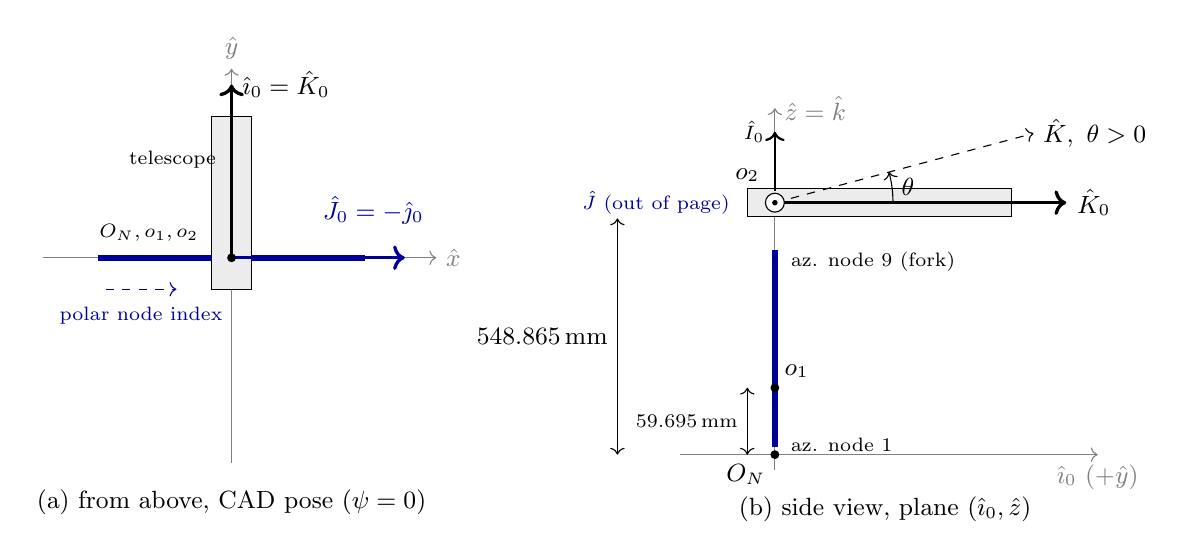
\begin{tikzpicture}[font=\small]
\begin{scope}
\draw[->, gray] (-2.4,0) -- (2.6,0) node[right] {$\hat x$};
\draw[->, gray] (0,-2.6) -- (0,2.4) node[above] {$\hat y$};
\draw[fill=gray!15] (-0.250,-0.400) -- (-0.250,1.800) -- (0.250,1.800) -- (0.250,-0.400) -- cycle;
\node[font=\scriptsize] at (-0.750,1.250) {telescope};
\draw[line width=2.2pt, blue!60!black] (-1.700,0.000) -- (-0.250,0.000);
\draw[line width=2.2pt, blue!60!black] (0.250,0.000) -- (1.700,0.000);
\draw[very thick, ->] (0,0) -- (0.000,2.200) node[anchor=west] {$\hat\imath_0 = \hat K_0$};
\draw[very thick, ->, blue!60!black] (0,0) -- (2.200,0.000);
\node[blue!60!black, anchor=south] at (1.800,0.300) {$\hat J_0 = -\hat\jmath_0$};
\draw[->, blue!60!black, dashed] (-1.600,-0.400) -- ++(-0.000:0.9);
\node[blue!60!black, font=\scriptsize, anchor=north] at (-1.150,-0.500) {polar node index};
\fill (0,0) circle (1.6pt);
\node[anchor=south east, font=\scriptsize] at (-0.300,0.080) {$O_N, o_1, o_2$};
\node at (0,-3.1) {(a) from above, CAD pose ($\psi = 0$)};
\end{scope}
\begin{scope}[xshift=6.9cm, yshift=-2.5cm]
\draw[->, gray] (-1.2,0) -- (4.1,0) node[below] {$\hat\imath_0$ $(+\hat{y})$};
\draw[->, gray] (0,-0.2) -- (0,4.4) node[right] {$\hat z = \hat k$};
\fill (0,0) circle (1.6pt) node[below left] {$O_N$};
\draw[line width=2.2pt, blue!60!black] (0,0.1) -- (0,2.600);
\fill (0.000,0.850) circle (1.6pt) node[above right] {$o_1$};
\node[right, font=\scriptsize] at (0.08,2.450) {az. node 9 (fork)};
\node[right, font=\scriptsize] at (0.08,0.12) {az. node 1};
\draw[fill=gray!15, rotate around={-0.000:(0,3.2)}] (-0.35,3.02) rectangle (3.0,3.3800000000000003);
\draw[very thick, ->, rotate around={-0.000:(0,3.2)}] (0,3.2) -- (3.7,3.2) node[right] {$\hat K_0$};
\draw[dashed, ->] (0,3.2) -- ++(15:3.4) node[right] {$\hat K,\ \theta>0$};
\draw[thick, ->] (0,3.2) ++(0.0,0.15) -- ++(0,0.75) node[left, font=\scriptsize] {$\hat I_0$};
\draw[->] (1.5,3.2) arc (0:15:1.5) node[midway, right] {$\theta$};
\draw[fill=white] (0,3.2) circle (0.12); \fill (0,3.2) circle (0.035);
\node at (-0.35,3.5500000000000003) {$o_2$};
\node[blue!60!black, font=\scriptsize, anchor=east] at (-0.45,3.2) {$\hat J$ (out of page)};
\draw[<->] (-2.0,0) -- (-2.0,3.0) node[midway, left] {$548.865$\,mm};
\draw[<->] (-0.35,0) -- (-0.35,0.850) node[midway, left, font=\scriptsize] {$59.695$\,mm};
\node at (1.4,-0.7) {(b) side view, plane $(\hat\imath_0, \hat z)$};
\end{scope}
\end{tikzpicture}}
\caption{CAD pose of the mount, drawn from the data of \texttt{frames}. (a) View from above: telescope along $\hat\imath_0 = \hat K_0$, polar shaft along $\hat J_0 = -\hat\jmath_0$ (blue) with the direction of increasing polar node index; $O_N$, $o_1$, $o_2$ project onto the same point. (b) Side view in the vertical plane of the pointing direction: origins $O_N$, $o_1$, $o_2$ on $\hat z$, azimuth shaft from node 1 to node 9 (fork), $\hat I_0$ upwards, $\hat J$ out of the page, $\theta>0$ raising the pointing.}\label{fig:frames}
\end{figure}

\subsection{Eccentricities, telescope tensor and gravity}\label{subsec:eccentricity}
The centre of mass of each body has an eccentricity with respect to its centre of rotation:
\begin{gather}
\mathbf e_1 = \mathbf r_{G_1} - \mathbf r_{o_1}\ \text{(fork, in frame 1)}, \qquad \mathbf d_2 = [d_I,\ d_J,\ d_K]^{\mathsf T} = \mathbf R_{N2}^{(0)\mathsf T}\bigl(\mathbf r_{G_2} - \mathbf r_{o_2}\bigr)\ \text{(telescope, in frame 2)}.
\end{gather}
The fork turns only about $\hat k$ and enters through its moment of inertia about the azimuth axis, $J_1 = I_{zz,G_1} + m_1(e_{1,x}^2 + e_{1,y}^2)$. The telescope tensor is exported from Onshape about $G_2$ with axes parallel to $N$, then transported to $o_2$ and rotated into frame 2 (tensor convention, $I_{ab} = -\int a\,b\,dm$ for $a \ne b$; $\mathbf I_3$ is the $3\times3$ identity):
\begin{gather}
\mathbf r = \mathbf r_{G_2} - \mathbf r_{o_2},\qquad \mathbf I_{p,o_2}\big|_N = \mathbf I_{p,G_2}\big|_N + m_p\bigl(\|\mathbf r\|^2\mathbf I_3 - \mathbf r\,\mathbf r^{\mathsf T}\bigr),\qquad \mathbf I_{p,o_2}\big|_2 = \mathbf R_{N2}^{(0)\mathsf T}\,\mathbf I_{p,o_2}\big|_N\,\mathbf R_{N2}^{(0)},
\end{gather}
whose components along $\hat I, \hat J, \hat K$ are $I_{II}, I_{JJ}, I_{KK}, I_{IJ}, I_{IK}, I_{JK}$. With the Onshape data of the telescope ($m_p = 16.61$\,kg),
\begin{gather}
\mathbf I_{p,o_2}\big|_2 = \begin{bmatrix}0.87307 & 7.13\times10^{-7} & -0.0075079 \\ 7.13\times10^{-7} & 0.88146 & -1.14\times10^{-6} \\ -0.0075079 & -1.14\times10^{-6} & 0.28454\end{bmatrix}\ \text{kg\,m}^2,\qquad \mathbf d_2 = \begin{bmatrix}-4.79\\ -0.0005\\ 67.39\end{bmatrix}\ \text{mm}.
\end{gather}
$I_{JJ} = 0.8815$\,kg\,m$^2$ is the inertia of the telescope about the polar axis. Gravity acts on the telescope with the moment about $\hat J$ and, linearised at $\theta_0$, the stiffness
\begin{gather}
M_{g,J}(\theta_p) = -m_p g\,\bigl(d_K\cos\theta_p - d_I\sin\theta_p\bigr),\qquad k_g = -\frac{\partial M_{g,J}}{\partial\theta_p}\Big|_{\theta_0} = -m_p g\,\bigl(d_I\cos\theta_0 + d_K\sin\theta_0\bigr),
\end{gather}
so $k_g = \kgSeven$\,N\,m/rad at $\theta_0 = 0$: gravity is negligible against the shaft stiffnesses, and only produces a very low pole ($\approx 0.15$\,Hz) in the polar responses.

%% ---------------------------------------------------------------------------------------------------
\section{Input geometry}\label{sec:geometry}
The geometry of each axis is entered in \texttt{config.yaml} as a sequence of elements, each made of coaxial layers (solid or hollow cylinders, steel or aluminium) or given as CAD data. Figures~\ref{fig:geom_az} and~\ref{fig:geom_pol} show the shafts as entered; the telescope has no shaft through it, so polar element 3 only joins the two bearing seats. The azimuth fork (with the polar shafts) and the telescope are entered as rigid bodies from the Onshape mass properties.
\begin{figure}[H]\centering
\includegraphics[width=0.95\linewidth]{figures/geometria_azimut.pdf}
\caption{Azimuth shaft as entered (nodes $1\dots9$, elements e1--e8).}\label{fig:geom_az}\end{figure}
\begin{figure}[H]\centering
\includegraphics[width=0.95\linewidth]{figures/geometria_polare.pdf}
\caption{Polar shaft as entered (nodes $1\dots11$; the telescope joins nodes 3 and 4 at P; elements e2 and e4 run in the bearings).}\label{fig:geom_pol}\end{figure}

%% ---------------------------------------------------------------------------------------------------
\section{Element properties}\label{sec:elements}
For a layer of length $L$, outer and inner diameters $D_o$, $D_i$, density $\rho$ and shear modulus $G$ (steel $\rho = 8000$\,kg/m$^3$, $G = 77$\,GPa; aluminium $\rho = 2810$\,kg/m$^3$, $G = 26.9$\,GPa):
\begin{gather}
m = \rho\,\frac{\pi}{4}\left(D_o^2 - D_i^2\right)L, \qquad J = \frac{\pi\rho L}{32}\left(D_o^4 - D_i^4\right), \qquad J_p = \frac{\pi}{32}\left(D_o^4 - D_i^4\right).
\end{gather}
Coaxial layers add their inertias and act in parallel; the segments of an element add their inertias and act in series:
\begin{gather}
k_s = \frac{1}{L_s}\sum_{\ell\ \text{carrying}} G_\ell J_{p,\ell}, \qquad \frac{1}{k_e} = \sum_s \frac{1}{k_s} + \frac{1}{k_{joint}}, \qquad J_e = \sum_s\sum_\ell J_{s\ell}.
\end{gather}
Tables~\ref{tab:el_az} and~\ref{tab:el_pol} give the totals per element. No joint compliance ($k_{joint}$) is modelled: shrink fits, keys and flanges are assumed rigid.
\begin{table}[H]\centering\small
\caption{Azimuth elements: length $L$ [mm], mass $m$ [g], inertia $J_e$ [kg\,m$^2$], stiffness $k_e$ [N\,m/rad].}\label{tab:el_az}
\begin{tabular}{rrrrr}\toprule el. & $L$ & $m$ & $J_e$ & $k_e$ \\ \midrule
1 & 29 & 46.65 & $1.49\times10^{-6}$ & $1.71\times10^{4}$ \\
2 & 20 & 446.3 & $3.46\times10^{-4}$ & $8.28\times10^{6}$ \\
3 & 22.59 & 36.34 & $1.16\times10^{-6}$ & $2.19\times10^{4}$ \\
4 & 10 & 103.9 & $2.15\times10^{-5}$ & $2.07\times10^{6}$ \\
5 & 10 & 103.9 & $2.15\times10^{-5}$ & $2.07\times10^{6}$ \\
6 & 30.88 & 49.67 & $1.59\times10^{-6}$ & $1.60\times10^{4}$ \\
7 & 35.53 & 139.5 & $1.09\times10^{-5}$ & $8.31\times10^{4}$ \\
8 & 17.5 & 134.7 & $2.06\times10^{-5}$ & $6.48\times10^{5}$
\\ \bottomrule\end{tabular}\end{table}
\begin{table}[H]\centering\small
\caption{Polar elements, baseline configuration (element 3 is the telescope seat, without shaft).}\label{tab:el_pol}
\begin{tabular}{rrrrr}\toprule el. & $L$ & $m$ & $J_e$ & $k_e$ \\ \midrule
1 & 58.29 & 228.9 & $1.79\times10^{-5}$ & $5.07\times10^{4}$ \\
2 & 15.32 & 238.6 & $2.10\times10^{-4}$ & $8.58\times10^{6}$ \\
3 & 60 & 0 & $0$ & -- \\
4 & 17.38 & 270.6 & $2.39\times10^{-4}$ & $7.57\times10^{6}$ \\
5 & 47.9 & 77.05 & $2.47\times10^{-6}$ & $1.03\times10^{4}$ \\
6 & 10.5 & 109.3 & $2.26\times10^{-5}$ & $1.98\times10^{6}$ \\
7 & 10.5 & 109.3 & $2.26\times10^{-5}$ & $1.98\times10^{6}$ \\
8 & 38.74 & 62.31 & $1.99\times10^{-6}$ & $1.28\times10^{4}$ \\
9 & 27 & 1309 & $1.26\times10^{-3}$ & $1.67\times10^{7}$ \\
10 & 12.08 & 19.44 & $6.22\times10^{-7}$ & $4.10\times10^{4}$
\\ \bottomrule\end{tabular}\end{table}

%% ---------------------------------------------------------------------------------------------------
\section{FEM and modal truncation}\label{sec:fem}
\paragraph{Torsional FEM.} Each axis is a chain of two-node torsional elements, 8 for the azimuth and 10 for the polar axis (polar element 3, the telescope seat, has no shaft and joins nodes 3 and 4 into P), with element matrices
\begin{gather}
\mathbf K_e = k_e\begin{bmatrix}1&-1\\-1&1\end{bmatrix}, \qquad \mathbf M_e = \frac{J_e}{6}\begin{bmatrix}2&1\\1&2\end{bmatrix}\ \ \text{(consistent mass, uniform element)},
\end{gather}
assembled on the shared nodes; concentrated inertias (fork, rotors) are added on the diagonal. Damping is $\mathbf C = \beta\mathbf K + \mathbf C_b$ with $\beta$ set so that $\zeta = 0.01$ on the first flexible mode of each axis (placeholder), $\mathbf C_b$ the bearing friction (zero here). The checks are $\mathbf K\mathbf 1 = \mathbf 0$ (one rigid mode per axis), $\mathbf M \succ 0$ and $\mathbf 1^{\mathsf T}\mathbf M\mathbf 1 = \sum_e J_e + \sum J^n$. The azimuth has 9 nodes, the polar axis 10 (P included). The two axes are coupled as described in Section~\ref{subsec:coupling}.
\paragraph{Modal truncation (Gawronski).} For each axis the FEM is solved with the telescope frozen at its attachment node, i.e.\ with the mass matrix $\bar{\mathbf M}$ equal to $\mathbf M$ plus the telescope inertia about the axis on the diagonal entry of the attachment node (the fork node L $=$ azimuth node 9, the telescope node P):
\begin{gather}
(\mathbf K - \omega_i^2\bar{\mathbf M})\boldsymbol\phi_i = \mathbf 0, \qquad \boldsymbol\Phi = [\mathbf 1,\ \boldsymbol\phi_1,\ \dots,\ \boldsymbol\phi_k], \qquad \boldsymbol\Phi^{\mathsf T}\bar{\mathbf M}\boldsymbol\Phi = \operatorname{diag}(J_{tot}, 1, \dots, 1),
\end{gather}
and the rigid mode plus the flexible modes in the band of interest ($f \le 2f_{band}$, $f_{band} = 2000$\,Hz) are kept; each retained mode keeps its frequency, shape and damping exactly. A validation loop compares the truncated model with the 18-element FEM at every operating point and adds the discarded mode with the largest Hankel norm if needed (here one azimuth mode). Table~\ref{tab:modes} lists the modes of the 18-element FEM; the truncated model agrees with it within $0.018$\,dB and $0.06^\circ$ on the encoder channels, and the excluded zeros within $10^{-4}$ in relative frequency.
\begin{table}[H]\centering\small
\caption{Modes of the 18-element FEM of each axis (baseline configuration, consistent mass, telescope frozen): frequency, damping, Hankel norm [rad/(N\,m)] and truncation outcome.}\label{tab:modes}
\begin{tabular}{llrrrl}\toprule axis & mode & $f$ [Hz] & $\zeta$ & $\|G_i\|_h$ & \\ \midrule
azimuth & 0 & $0$ & $0$ & $\infty$ & kept \\
azimuth & 1 & $752.2$ & $0.01$ & $0.002$ & kept \\
azimuth & 2 & $4595$ & $0.061$ & $9.1\times10^{-6}$ & kept \\
azimuth & 3 & $2.134\times10^{4}$ & $0.28$ & $1.1\times10^{-10}$ & no \\
azimuth & 4 & $2.952\times10^{4}$ & $0.39$ & $2.4\times10^{-9}$ & no \\
polar & 0 & $0$ & $0$ & $\infty$ & kept \\
polar & 1 & $335.6$ & $0.01$ & $3.6\times10^{-6}$ & kept \\
polar & 2 & $3557$ & $0.11$ & $2.7\times10^{-9}$ & kept \\
polar & 3 & $1.457\times10^{4}$ & $0.43$ & $5.7\times10^{-12}$ & no \\
polar & 4 & $4.886\times10^{4}$ & $1.5$ & $2.1\times10^{-13}$ & no
\\ \bottomrule\end{tabular}\end{table}
\subsection{Coupling between the axes}\label{subsec:coupling}
The whole polar axis is carried by the fork, so every polar node $i$ turns with the angular velocity $\boldsymbol\omega_i = \dot\psi_L\hat k + \dot\theta_i\hat J$, with $\hat k\perp\hat J$. For an axisymmetric node (shaft segment, rotor) with axial inertia $J_i$, transverse inertia $I_{t,i}$ and distance $y_i$ from the azimuth axis, the kinetic energy has no cross term,
\begin{gather}
T_i = \tfrac12 J_i\dot\theta_i^2 + \tfrac12\bigl(I_{t,i} + m_i y_i^2\bigr)\dot\psi_L^2,\qquad J^{ax} = \sum_i\bigl(I_{t,i} + m_i y_i^2\bigr),
\end{gather}
so the polar shafts add the constant inertia $J^{ax}$ to the azimuth load. Here $J^{ax}$ is already contained in the CAD tensor of the fork, which includes the polar shafts, and is not added again. The telescope is not axisymmetric about $\hat J$: with $\boldsymbol\omega_p\big|_2 = [\dot\psi_L\cos\theta_p,\ \dot\theta_p,\ \dot\psi_L\sin\theta_p]^{\mathsf T}$ (Section~\ref{sec:frames}),
\begin{gather}
T_p = \tfrac12\boldsymbol\omega_p^{\mathsf T}\,\mathbf I_{p,o_2}\big|_2\,\boldsymbol\omega_p = \tfrac12 J_{\psi,p}(\theta_p)\,\dot\psi_L^2 + M_{12}(\theta_p)\,\dot\psi_L\dot\theta_p + \tfrac12 I_{JJ}\,\dot\theta_p^2,\\
J_{\psi,p}(\theta_p) = I_{II}\cos^2\theta_p + I_{IK}\sin 2\theta_p + I_{KK}\sin^2\theta_p,\qquad M_{12}(\theta_p) = I_{IJ}\cos\theta_p + I_{JK}\sin\theta_p .
\end{gather}
The kinetic energy of the model is $T = \tfrac12\dot{\mathbf q}_\psi^{\mathsf T}\mathbf M_\psi\dot{\mathbf q}_\psi + \tfrac12 J^{ax}\dot\psi_L^2 + \tfrac12\dot{\mathbf q}_\theta^{\mathsf T}\mathbf M_\theta\dot{\mathbf q}_\theta + T_p$, with $\mathbf q_\psi$, $\mathbf q_\theta$ the rotations of the nodes of the two axes and $\mathbf M_\psi$, $\mathbf M_\theta$ their mass matrices (those of the 18-element FEM here, those of the 7-DOF model in Section~\ref{sec:lumped}). The stator of the polar motor is on the fork: the reaction of $\tau_\theta$ acts about $\hat J\perp\hat k$ and does no work on $\psi_L$; the gyroscopic moments of the axisymmetric polar nodes are orthogonal to $\hat J$ and are carried by the bearings.
\subsection{Results of the 18-element FEM}\label{subsec:fem_results}
Figure~\ref{fig:fem_modes7} shows the flexible modes in the band. The first azimuth mode ($\fAzPoleFemSeven$\,Hz) is the drive side (encoder and motor) oscillating against the heavy fork, which stays almost still; the first polar mode ($\fpFemSevenOne$\,Hz) is the motor and rear end oscillating against the telescope, which stays almost still at P. The second modes are local (a few light shaft segments) and lie above 3\,kHz.
\begin{figure}[H]\centering
\includegraphics[width=\linewidth]{figures/fem_modes_7.pdf}
\caption{Flexible modes of the 18-element FEM in the band, baseline configuration (telescope frozen, $\theta_0 = 0$): normalised shape against the position along the shaft, with encoder, motor and attachment node (fork L, telescope P).}\label{fig:fem_modes7}\end{figure}
To compare the FEM with the measurements, the two axes of the 18-element FEM are coupled (9 azimuth and 10 polar coordinates, no reduction), linearised at $\theta_0 = 0$ and evaluated in the units of the measurement, eq.~\eqref{eq:plant} (Figure~\ref{fig:fem_frf7}). In the encoder channel the FEM has the azimuth load antiresonance at $\fAzZeroFemSeven$\,Hz (measured $\fAzZeroMeas$\,Hz), but on the polar axis it has no zero below $\fzFemSevenEnc$\,Hz: an antiresonance close to the measured $\fzMeas$\,Hz appears only in the motor channel ($\fzSevenMotor$\,Hz), which is not the measured one. These results are discussed in Section~\ref{sec:cmp7} with the reduced model, whose elements map directly onto the physical components.
\begin{figure}[H]\centering
\includegraphics[width=\linewidth,height=0.62\textheight,keepaspectratio]{figures/fem_frf_7.pdf}
\caption{18-element FEM, baseline configuration, in the units of the measurement: $j\omega K_t\,\theta/\tau$ at the encoder (blue, measured channel) and at the motor (orange, dashed), against the measurements (black); azimuth, polar with and without the telescope. Dotted vertical lines: poles of the model.}\label{fig:fem_frf7}\end{figure}

%% ---------------------------------------------------------------------------------------------------
\section{The 7-DOF model}\label{sec:lumped}
\paragraph{Degrees of freedom and elements.} The 7-DOF model is a reduced model of the 18-element FEM. Only the nodes where something is applied, measured or attached are kept: encoder, motor and fork on the azimuth; encoder, telescope node P, motor and rear end on the polar axis. Each kept node becomes a \emph{lumped inertia} and its rotation is one \emph{degree of freedom}; the FEM elements between two kept nodes are condensed into one \emph{equivalent element}, a massless spring with
\begin{gather}
\frac{1}{k_{eq}} = \sum_i\frac{1}{k_i}\quad\text{(springs in series)},\qquad J_{eq} = \sum_i J_i,\qquad c_{eq} = \beta k_{eq},
\end{gather}
whose inertia $J_{eq}$ is split in halves between its two end nodes. Each lumped inertia is therefore its concentrated inertia (fork) plus half of the adjacent equivalent elements. The model has 7 degrees of freedom, $\mathbf q = [\psi_e,\ \psi_m,\ \psi_L,\ \theta_e,\ \theta_p,\ \theta_m,\ \theta_r]^{\mathsf T}$, and 5 equivalent elements (Figure~\ref{fig:chain7}, Tables~\ref{tab:lump7_el} and~\ref{tab:lump7_nd}).
\begin{figure}[H]\centering
\resizebox{\linewidth}{!}{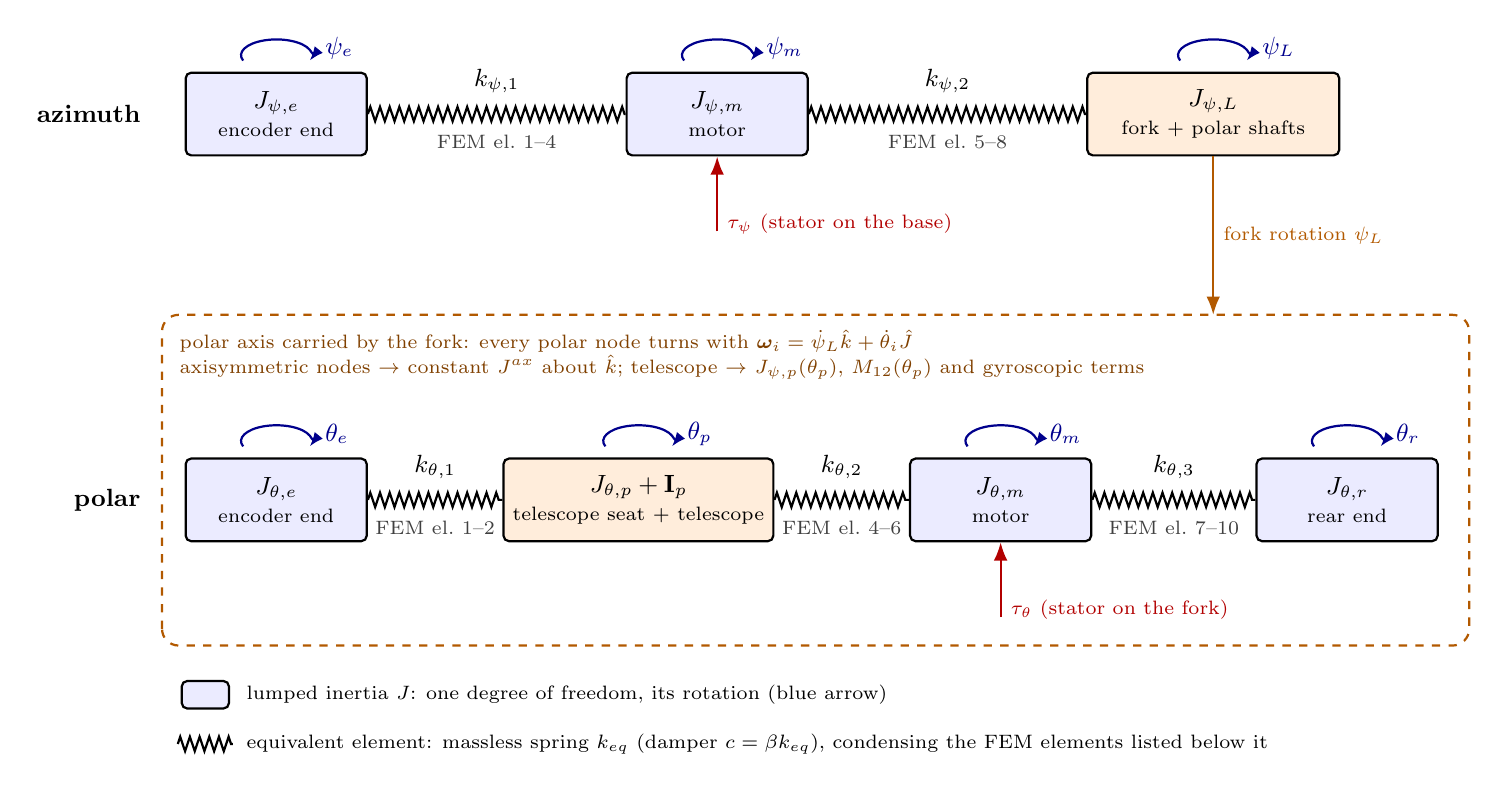
\begin{tikzpicture}[font=\small,
 dof/.style={draw, thick, rounded corners=2pt, minimum width=2.3cm, minimum height=1.05cm, align=center, fill=blue!8},
 spr/.style={decorate, decoration={zigzag, segment length=3.5pt, amplitude=2.6pt}, thick},
 rot/.style={-{Latex[length=1.8mm]}, thick, blue!55!black}]
% ---- azimuth
\node[dof] (pe) at (0,0) {$J_{\psi,e}$\\[-1pt] {\scriptsize encoder end}};
\node[dof] (pm) at (5.6,0) {$J_{\psi,m}$\\[-1pt] {\scriptsize motor}};
\node[dof, fill=orange!14, minimum width=3.2cm] (pL) at (11.9,0) {$J_{\psi,L}$\\[-1pt] {\scriptsize fork + polar shafts}};
\draw[spr] (pe.east) -- node[above=4pt] {$k_{\psi,1}$} node[below=4pt, font=\scriptsize, gray!50!black] {FEM el.\ 1--4} (pm.west);
\draw[spr] (pm.east) -- node[above=4pt] {$k_{\psi,2}$} node[below=4pt, font=\scriptsize, gray!50!black] {FEM el.\ 5--8} (pL.west);
\foreach \n/\q in {pe/\psi_e, pm/\psi_m, pL/\psi_L} {
  \draw[rot] ($(\n.north)+(-0.42,0.14)$) arc[start angle=200, end angle=-20, x radius=0.45, y radius=0.2];
  \node[blue!55!black, anchor=west] at ($(\n.north)+(0.5,0.3)$) {$\q$};}
\draw[-{Latex}, thick, red!70!black] ($(pm.south)+(0,-0.95)$) -- (pm.south) node[pos=0.1, right, font=\scriptsize] {$\tau_\psi$ (stator on the base)};
\node[anchor=east] at (-1.6,0) {\textbf{azimuth}};
% ---- polar axis, carried by the fork
\draw[dashed, thick, orange!70!black, rounded corners=6pt] (-1.45,-6.75) rectangle (15.15,-2.55);
\node[anchor=north west, font=\scriptsize, align=left, orange!50!black] at (-1.35,-2.62) {polar axis carried by the fork: every polar node turns with $\boldsymbol\omega_i = \dot\psi_L\hat k + \dot\theta_i\hat J$\\ axisymmetric nodes $\to$ constant $J^{ax}$ about $\hat k$; telescope $\to$ $J_{\psi,p}(\theta_p)$, $M_{12}(\theta_p)$ and gyroscopic terms};
\draw[-{Latex}, thick, orange!70!black] (pL.south) -- node[right, font=\scriptsize] {fork rotation $\psi_L$} (11.9,-2.55);
\node[dof] (te) at (0,-4.9) {$J_{\theta,e}$\\[-1pt] {\scriptsize encoder end}};
\node[dof, fill=orange!14, minimum width=2.7cm] (tp) at (4.6,-4.9) {$J_{\theta,p} + \mathbf I_p$\\[-1pt] {\scriptsize telescope seat + telescope}};
\node[dof] (tm) at (9.2,-4.9) {$J_{\theta,m}$\\[-1pt] {\scriptsize motor}};
\node[dof] (tr) at (13.6,-4.9) {$J_{\theta,r}$\\[-1pt] {\scriptsize rear end}};
\draw[spr] (te.east) -- node[above=4pt] {$k_{\theta,1}$} node[below=4pt, font=\scriptsize, gray!50!black] {FEM el.\ 1--2} (tp.west);
\draw[spr] (tp.east) -- node[above=4pt] {$k_{\theta,2}$} node[below=4pt, font=\scriptsize, gray!50!black] {FEM el.\ 4--6} (tm.west);
\draw[spr] (tm.east) -- node[above=4pt] {$k_{\theta,3}$} node[below=4pt, font=\scriptsize, gray!50!black] {FEM el.\ 7--10} (tr.west);
\foreach \n/\q in {te/\theta_e, tp/\theta_p, tm/\theta_m, tr/\theta_r} {
  \draw[rot] ($(\n.north)+(-0.42,0.14)$) arc[start angle=200, end angle=-20, x radius=0.45, y radius=0.2];
  \node[blue!55!black, anchor=west] at ($(\n.north)+(0.5,0.3)$) {$\q$};}
\draw[-{Latex}, thick, red!70!black] ($(tm.south)+(0,-0.95)$) -- (tm.south) node[pos=0.1, right, font=\scriptsize] {$\tau_\theta$ (stator on the fork)};
\node[anchor=east] at (-1.6,-4.9) {\textbf{polar}};
% ---- legend
\draw[thick, rounded corners=2pt, fill=blue!8] (-1.2,-7.55) rectangle (-0.6,-7.2);
\node[anchor=west, font=\scriptsize] at (-0.5,-7.38) {lumped inertia $J$: one degree of freedom, its rotation (blue arrow)};
\draw[spr] (-1.25,-8.0) -- (-0.55,-8.0);
\node[anchor=west, font=\scriptsize] at (-0.5,-8.0) {equivalent element: massless spring $k_{eq}$ (damper $c = \beta k_{eq}$), condensing the FEM elements listed below it};
\end{tikzpicture}}
\caption{7-DOF model. Each box is a lumped inertia and carries one degree of freedom, its rotation; each zigzag is an equivalent element (massless spring) condensing the listed FEM elements. The whole polar axis is mounted on the fork (dashed frame): its nodes turn with the fork rotation $\psi_L$ as well as with their own $\theta_i$. Orange: bodies carrying the fork and telescope tensors.}\label{fig:chain7}\end{figure}
\begin{table}[H]\centering\small
\caption{7-DOF model, equivalent elements: physical components, end nodes, FEM elements condensed, inertia $J_{eq}$ [kg\,m$^2$] and series stiffness $k_{eq}$ [N\,m/rad].}\label{tab:lump7_el}
\begin{tabularx}{\linewidth}{lYlL{0.12\linewidth}rr}\toprule element & component & nodes & FEM el. & $J_{eq}$ & $k_{eq}$ \\ \midrule
$k_{\psi,1}$ & shaft with flange, encoder to motor & 1--5 & 1 2 3 4 & $3.70\times10^{-4}$ & $9.55\times10^{3}$ \\
$k_{\psi,2}$ & shaft, motor to fork & 5--9 & 5 6 7 8 & $5.46\times10^{-5}$ & $1.31\times10^{4}$ \\
$k_{\theta,1}$ & encoder-side shaft and first bearing seat & 1--P & 1 2 & $2.28\times10^{-4}$ & $5.04\times10^{4}$ \\
$k_{\theta,2}$ & second bearing seat and shaft up to the motor & P--7 & 4 5 6 & $2.64\times10^{-4}$ & $1.03\times10^{4}$ \\
$k_{\theta,3}$ & shaft, motor to rear end & 7--11 & 7 8 9 10 & $1.29\times10^{-3}$ & $9.69\times10^{3}$
\\ \bottomrule\end{tabularx}\end{table}
\begin{table}[H]\centering\small
\caption{7-DOF model, lumped inertias (one per degree of freedom) [kg\,m$^2$]: concentrated inertia plus half of the adjacent equivalent elements. The telescope tensor ($m_p = 16.61$\,kg, $I_{JJ} = 0.8815$\,kg\,m$^2$) is not included: it enters through its own terms (Section~\ref{subsec:coupling}).}\label{tab:lump7_nd}
\begin{tabularx}{\linewidth}{lYlr}\toprule inertia & component & node & $J$ \\ \midrule
$J_{\psi,e}$ & encoder end of the azimuth shaft & 1 & $1.85\times10^{-4}$ \\
$J_{\psi,m}$ & motor node, torque $\tau_\psi$ & 5 & $2.12\times10^{-4}$ \\
$J_{\psi,L}$ & load: fork and polar shafts (CAD); telescope through its tensor & 9 & $1.25$ \\
$J_{\theta,e}$ & encoder end of the polar shaft & 1 & $1.14\times10^{-4}$ \\
$J_{\theta,p}$ & telescope seat P, rigid telescope & P & $2.46\times10^{-4}$ \\
$J_{\theta,m}$ & motor node, torque $\tau_\theta$ & 7 & $7.76\times10^{-4}$ \\
$J_{\theta,r}$ & rear end of the polar shaft & 11 & $6.44\times10^{-4}$
\\ \bottomrule\end{tabularx}\end{table}
\subsection{Newton--Euler equations}\label{subsec:ne7}
Each degree of freedom gets a moment balance on its lumped inertia. The torque transmitted by an equivalent element, positive on its second node, is
\begin{gather}
T_{\psi,1} = k_{\psi,1}(\psi_e - \psi_m) + c_{\psi,1}(\dot\psi_e - \dot\psi_m),\qquad T_{\psi,2} = k_{\psi,2}(\psi_m - \psi_L) + c_{\psi,2}(\dot\psi_m - \dot\psi_L),\\
T_{\theta,1} = k_{\theta,1}(\theta_e - \theta_p) + c_{\theta,1}(\dot\theta_e - \dot\theta_p),\qquad T_{\theta,2} = k_{\theta,2}(\theta_p - \theta_m) + c_{\theta,2}(\dot\theta_p - \dot\theta_m),\\
T_{\theta,3} = k_{\theta,3}(\theta_m - \theta_r) + c_{\theta,3}(\dot\theta_m - \dot\theta_r),
\end{gather}
and $b\,\dot q$ is the viscous friction of a bearing (azimuth: to the ground; polar: to the fork; zero in the current data). With $'$ denoting $d/d\theta_p$ and $M_{g,J}$ the gravity moment of Section~\ref{subsec:eccentricity}, the nonlinear equations are
\begin{gather}
(\psi_e)\quad J_{\psi,e}\,\ddot\psi_e = -T_{\psi,1} - b_{\psi,e}\dot\psi_e, \label{eq:ne_psie}\\
(\psi_m)\quad J_{\psi,m}\,\ddot\psi_m = \tau_\psi + T_{\psi,1} - T_{\psi,2} - b_{\psi,m}\dot\psi_m, \label{eq:ne_psim}\\
(\psi_L)\quad \bigl[J_{\psi,L} + J^{ax} + J_{\psi,p}(\theta_p)\bigr]\ddot\psi_L + M_{12}(\theta_p)\,\ddot\theta_p + J_{\psi,p}'(\theta_p)\,\dot\psi_L\dot\theta_p + M_{12}'(\theta_p)\,\dot\theta_p^2 = T_{\psi,2} - b_{\psi,L}\dot\psi_L, \label{eq:ne_psiL}\\
(\theta_e)\quad J_{\theta,e}\,\ddot\theta_e = -T_{\theta,1} - b_{\theta,e}\dot\theta_e, \label{eq:ne_the}\\
(\theta_p)\quad \bigl[J_{\theta,p} + I_{JJ}\bigr]\ddot\theta_p + M_{12}(\theta_p)\,\ddot\psi_L - \tfrac12 J_{\psi,p}'(\theta_p)\,\dot\psi_L^2 = T_{\theta,1} - T_{\theta,2} + M_{g,J}(\theta_p) - b_{\theta,p}\dot\theta_p, \label{eq:ne_thp}\\
(\theta_m)\quad J_{\theta,m}\,\ddot\theta_m = \tau_\theta + T_{\theta,2} - T_{\theta,3} - b_{\theta,m}\dot\theta_m, \label{eq:ne_thm}\\
(\theta_r)\quad J_{\theta,r}\,\ddot\theta_r = T_{\theta,3} - b_{\theta,r}\dot\theta_r. \label{eq:ne_thr}
\end{gather}
The only nonlinearities are the trigonometric functions of $\theta_p$ and the velocity products: $J_{\psi,p}'\dot\psi_L\dot\theta_p$ (Coriolis, on the azimuth), $-\tfrac12 J_{\psi,p}'\dot\psi_L^2$ (centrifugal, on the polar axis) and $M_{12}'\dot\theta_p^2$ (from the products of inertia). The equations are derived symbolically from the moment balances and checked against Lagrange's equations with the kinetic energy of Section~\ref{subsec:coupling} (difference identically zero). The model is linearised at each elevation $\theta_0$, where gravity enters as the stiffness $k_g$.
\subsection{Zeros and poles}\label{subsec:zeros7}
The poles are the free modes of the whole structure and are common to every channel. The zeros depend on the actuator--sensor pair: they are the natural frequencies of the branches hanging off the actuator--sensor path, each with its attachment node clamped. Springs on the path add no zero, only a constant factor, and the number of zeros is $n - 1 - (\text{springs on the path})$, with $n$ the number of inertias. For the encoder channel of the 7-DOF polar chain (isolated axis, undamped) the path $\tau_\theta\to\theta_e$ crosses $k_{\theta,2}$ and $k_{\theta,1}$ and the only branch off it is the rear end:
\begin{gather}
\frac{\Theta_e}{T_\theta} = \frac{k_{\theta,1}k_{\theta,2}\,\bigl(J_{\theta,r}s^2 + k_{\theta,3}\bigr)}{\Delta(s)},\qquad \Delta(s) = \det\bigl(\mathbf M_\theta s^2 + \mathbf K_\theta\bigr)\ \text{(degree 8)}.\label{eq:tf7}
\end{gather}
\subsection{7-DOF model against the 18-element FEM}\label{subsec:lump_vs_fem7}
Table~\ref{tab:lump_fem7} compares the reduced model with the FEM it comes from. The zeros that depend on the light parts only through series stiffnesses (load antiresonance, telescope zero in the motor channel) are exact, and the first mode of each axis is 3--13\,\% higher, because the shaft inertia is concentrated at fewer nodes. The second modes are far too low ($\approx 0.3$--$0.4$ times the FEM value): above about 900\,Hz the 7-DOF model is not representative.
\begin{table}[H]\centering\small
\caption{Isolated axes (telescope frozen, $\theta_0 = 0$) and zeros of the coupled model: 18-element FEM against the 7-DOF model [Hz].}\label{tab:lump_fem7}
\begin{tabular}{lrrr}\toprule quantity & 18-element FEM & 7-DOF & difference [\%] \\ \midrule
azimuth, mode 1 & 752.2 & 774 & $+2.9$ \\
azimuth, mode 2 & 4595 & 1847 & $-59.8$ \\
polar, mode 1 & 335.6 & 379.5 & $+13.1$ \\
polar, mode 2 & 3557 & 943 & $-73.5$ \\
polar without telescope, mode 1 & 647.7 & 709.1 & $+9.5$ \\
zero $\tau_\psi\to\psi_e$ (load) & 12.49 & 12.49 & $0.0$ \\
zero $\tau_\theta\to\theta_e$, 1 & 504.5 & 617.4 & $+22.4$ \\
zero $\tau_\theta\to\theta_m$, 1 & 17.18 & 17.18 & $0.0$
\\ \bottomrule\end{tabular}\end{table}

%% ---------------------------------------------------------------------------------------------------
\section{Comparison of the 7-DOF model with the measurements}\label{sec:cmp7}
In Figures~\ref{fig:cmp7_az}--\ref{fig:cmp7_nt} the measured plant (black) is compared with the 7-DOF model at the encoder (blue, the measured channel) and, for reference, at the motor (orange, dashed). The model is linearised at $\theta_0 = 0$.
\begin{figure}[H]\centering
\includegraphics[width=\linewidth,height=0.42\textheight,keepaspectratio]{figures/cmp7_az.pdf}
\caption{Azimuth: 7-DOF model against measurement (3.5\,A).}\label{fig:cmp7_az}\end{figure}
\begin{figure}[H]\centering
\includegraphics[width=\linewidth,height=0.42\textheight,keepaspectratio]{figures/cmp7_pol.pdf}
\caption{Polar with telescope (4 screws): 7-DOF model against measurement (3.5\,A, 1--2000\,Hz).}\label{fig:cmp7_pol}\end{figure}
\begin{figure}[H]\centering
\includegraphics[width=\linewidth,height=0.42\textheight,keepaspectratio]{figures/cmp7_nt.pdf}
\caption{Polar without the telescope: 7-DOF model against measurement (2.5\,A).}\label{fig:cmp7_nt}\end{figure}
\begin{itemize}
\item \textbf{Azimuth.} The rigid-body line and the load antiresonance are reproduced: $\fAzZeroMeas$\,Hz measured against $\fAzZeroSeven$\,Hz (the fork oscillating on $k_{\psi,2}$ with encoder and motor still), and its shift with the elevation too. The first structural resonance is at $\fAzPoleMeas$\,Hz instead of the predicted $\fAzPoleSeven$\,Hz ($\fAzPoleFemSeven$\,Hz in the 18-element FEM).
\item \textbf{Polar with telescope.} The rigid-body line matches within about 1\,dB (5--11\,Hz), which confirms the units and the total inertia $J_{tot} = \Jtot$\,kg\,m$^2$. The measured encoder channel has a deep antiresonance at $\fzMeas$\,Hz, followed by a resonance at about $\fpMeas$\,Hz. The model has \emph{no zero below $\fzSevenEnc$\,Hz} in this channel \eqref{eq:tf7}, and neither has the 18-element FEM below $\fzFemSevenEnc$\,Hz: the zero at $\fzSevenMotor$\,Hz appears only in the motor channel, which is not the measured one.
\item \textbf{Polar without telescope.} The model is a free rigid inertia up to its first mode at $\fNtSeven$\,Hz ($\fNtFemSeven$\,Hz in the 18-element FEM); the measurement shows a first resonance at $\fNtPole$\,Hz, bracketed by antiresonances at $\fNtZeroOne$ and $\fNtZeroTwo$\,Hz.
\end{itemize}
The conclusion of this step is that the telescope cannot be rigidly attached on the shaft path between encoder and motor: the structure of the polar axis needs a branch hanging off that path.

%% ---------------------------------------------------------------------------------------------------
\section{Discrepancies and the new model}\label{sec:newmodel}
\subsection{Why a branch is needed}\label{subsec:branch}
An inertia added together with a spring \emph{on} the actuator--sensor path adds a pole and no zero. An inertia $I$ attached to the path through a spring $k$ \emph{off} the path adds one zero, at the natural frequency of that branch with its attachment node clamped, and the free structure has a pole after it, the shaft side oscillating against $I$. In a two-mass reduction, with everything on the shaft side of $k$ lumped in $J_{sh}$ and $J_{sh} + I = J_{tot}$ fixed by the rigid-body line,
\begin{gather}
\omega_z^2 = \frac{k + k_g}{I},\qquad \left(\frac{f_p}{f_z}\right)^2 \simeq 1 + \frac{I}{J_{sh}}.\label{eq:twomass}
\end{gather}
The measured zero ($\fzMeas$\,Hz) and pole (about $\fpMeas$\,Hz) give $I/J_{sh} = \ratioNeed$, i.e.\ $I = \JcNeed$\,kg\,m$^2$ and $J_{sh} = \JoneNeed$\,kg\,m$^2$ with $J_{tot} = \Jtot$\,kg\,m$^2$, and $k \approx \kbTwoMass$\,N\,m/rad. The only body of that size is the telescope ($I_{JJ} = 0.8815$\,kg\,m$^2$): the measured zero is the signature of the telescope hanging from a compliance off the shaft path.
\subsection{Hub, telescope interface and ring}\label{subsec:hub}
The polar axis is rebuilt as follows (Figure~\ref{fig:hubgeom}); the result is called the \emph{hub configuration}:
\begin{enumerate}
\item The \textbf{hub} (two side hubs and the support ring of the telescope) is part of the shaft path: it replaces polar elements 2, 3 and 4, its centre H carries the hub inertia, and its stiffness is the series of tube, flange and half ring on each side.
\item The \textbf{telescope is an external body}: it hangs from H through the interface stiffness $k_b$ (ring--telescope connection) and carries the telescope tensor, minus the tube section clamped in the ring, which belongs to the hub.
\item The \textbf{ring is stiffened}: the support ring is clamped to the side hubs through 16 threaded connections (8 per side) on curved flanges, which makes it much stiffer than the bare ring.
\end{enumerate}
\begin{figure}[H]\centering
\includegraphics[width=\linewidth]{figures/geometria_mozzo.pdf}
\caption{Hub and telescope geometry (mm): (a) view along the polar axis, side hubs and support ring (aluminium) with the telescope tube slid into the ring; (b) view along the telescope axis, the ring twisting and bending under the torque about $\hat J$; (c) springs in series along the polar axis (N\,m/rad) with the hub inertia at H and the telescope on $k_b$.}\label{fig:hubgeom}\end{figure}
\paragraph{Hub stiffness.} Each half of the hub is the series of the bearing-seat tube $\varnothing90/84\times42$, the flange $\varnothing90\times17$ and a half ring, all in aluminium:
\begin{gather}
k_{tube} = \frac{G\pi(D_o^4 - D_i^4)}{32L},\quad k_{flange} = \frac{G\pi D_o^4}{32L},\quad k_{ring}^{0} = \frac{4}{\pi R}\left(\frac{1}{EI_r} + \frac{1}{GJ_{tor}}\right)^{-1},\\
I_r = \frac{t b^3}{12},\quad J_{tor} = \chi\, b t^3,\quad \chi = \frac{1 - 0.63\,t/b + 0.052(t/b)^5}{3},\quad E = 2G(1+\nu),\\
\frac{1}{k_{half}} = \frac{1}{k_{tube}} + \frac{1}{k_{flange}} + \frac{1}{2\kappa_r k_{ring}^{0}},\qquad k_{hub} = \frac{k_{half}}{2}.
\end{gather}
$k_{ring}^{0}$ is the stiffness of the bare ring between its two attachment points, and each half of the hub carries half of its compliance; $\kappa_r$ is the stiffening factor. The ring ($\varnothing310/300\times100$, wall $t = 5$\,mm, width $b = 100$\,mm, mean radius $R = 152.5$\,mm, $\nu = 0.33$) is modelled as two half rings that twist (wall torsion, torsion constant $J_{tor}$ of the $t\times b$ rectangular section) and bend out of plane (second moment $I_r$), by Castigliano's theorem. Alone ($\kappa_r = 1$) it gives $k_{ring}^{0} = \kRingZero$\,N\,m/rad, by far the most compliant element of the hub; with $\kappa_r = \ringFactor$ the half ring contributes $2\kappa_r k_{ring}^{0} = \kRingHalf$\,N\,m/rad, against $k_{tube} = \kTube$ and $k_{flange} = \kFlange$, and the hub becomes $k_{half} = \kHalfHub$ ($k_{hub} = \kHub$\,N\,m/rad bearing to bearing, instead of $\kHubRingAlone$).
\paragraph{Hub and telescope inertias.} The hub inertia about the polar axis comes from the Onshape mass properties (side hubs and ring; $m = 2.054$\,kg, $0.0170$\,kg\,m$^2$, corrected by hand from the steel export to aluminium). The tube section $\varnothing300/290\times100$ clamped in the ring ($m = 1.30$\,kg, $0.0153$\,kg\,m$^2$) is moved from the telescope to the hub. Hence the hub node carries $J_{\theta,h} = \JhEight$\,kg\,m$^2$ and, in the hub configuration, $I_{JJ} = \JcEight$\,kg\,m$^2$ (CAD $0.8815$ minus $0.0153$). The hub is assumed not to be part of the fork CAD tensor (to be verified on the CAD): its inertia about $\hat z$ is added to $J^{ax}$ (Section~\ref{subsec:coupling}).
\paragraph{Free parameters.} Two stiffnesses of the hub configuration are not known from the CAD and are \emph{free parameters}, fitted on measurements (Table~\ref{tab:free}); all other values come from the geometry and the CAD.
\begin{table}[H]\centering\small
\caption{Free parameters of the hub configuration.}\label{tab:free}
\begin{tabularx}{\linewidth}{L{0.1\linewidth}L{0.22\linewidth}L{0.12\linewidth}Y}\toprule
parameter & meaning & value & fitted on \\ \midrule
$k_b$ & telescope--hub interface (ring--telescope connection) & $\kbCur$\,N\,m/rad & the measured zero at $\fzMeas$\,Hz and pole at about $\fpMeas$\,Hz, with the two-mass estimate \eqref{eq:twomass}; \emph{not} refitted after the hub inertias were introduced (the resulting zero is given in Section~\ref{sec:cmp8}) \\
$\kappa_r$ & multiplier of the half-ring stiffness (16 bolted connections on curved flanges) & $\ringFactor$ & the test without telescope, which shows no mode below about 400\,Hz, while the bare ring ($\kappa_r = 1$) gives a first mode at $\fNtEightRingOne$\,Hz \\ \bottomrule
\end{tabularx}\end{table}
\paragraph{Traceability.} The hub configuration (H4) was reached in four steps from the baseline, each kept in its own configuration and results folder (Table~\ref{tab:versions}).
\begin{table}[H]\centering\small
\caption{Versions of the model (folder \texttt{sim/gimbal\_multidof}); each configuration writes its results to the folder \texttt{results\_}\emph{name} (\texttt{results/} for the baseline). Only the baseline and the last version, H4, are compared in this report.}\label{tab:versions}
\begin{tabularx}{\linewidth}{L{0.085\linewidth}L{0.42\linewidth}Y}\toprule
version & configuration & change with respect to the previous one \\ \midrule
\textbf{baseline} & \texttt{config.yaml} & telescope rigidly attached at the shaft node P \\
H1 & \texttt{config\_hub.yaml} & hub on the shaft path (steel side hubs, support ring alone); telescope hung on the hub through $k_b$ \\
H2 & \texttt{config\_hub\_\allowbreak telescopeonring.yaml} & tube section clamped in the ring moved from the telescope to the hub \\
H3 & \texttt{config\_hub\_\allowbreak telescopeonring\_\allowbreak alhub.yaml} & side hubs in aluminium (material error in the CAD), hub tensor corrected \\
\textbf{H4} & \texttt{config\_hub\_\allowbreak telescopeonring\_\allowbreak alhub\_\allowbreak stiffring.yaml} & ring stiffness multiplied by $\kappa_r = \ringFactor$: the hub configuration of this report \\ \bottomrule
\end{tabularx}\end{table}
\subsection{FEM with hub}\label{subsec:femhub}
In the FEM the hub replaces polar elements 2, 3 and 4 with its two halves ($k_{half}$ each), which meet at the hub centre H; the telescope becomes a node P off the shaft, attached to H through $k_b$. The model keeps 18 elements (8 azimuth; 9 polar shaft elements and $k_b$) and is coupled and linearised as the 18-element FEM of Section~\ref{subsec:fem_results}. Its first polar mode ($\fpFemEightOne$\,Hz, Figure~\ref{fig:fem_modes8}) is the shaft, hub, encoder and motor oscillating against the telescope, which stays almost still: it is the pole after the telescope zero. The second ($\fpFemEightTwo$\,Hz) is the motor and rear end oscillating against the rest, as the first polar mode of the baseline configuration. In the encoder channel (Figure~\ref{fig:fem_frf8}) the telescope zero is now present, at $\fzFemEightEnc$\,Hz.
\begin{figure}[H]\centering
\includegraphics[width=\linewidth]{figures/fem_modes_8.pdf}
\caption{Flexible modes of the FEM with hub in the band, polar axis ($\theta_0 = 0$). The telescope (star) hangs from the hub centre H through $k_b$ (dashed).}\label{fig:fem_modes8}\end{figure}
\begin{figure}[H]\centering
\includegraphics[width=\linewidth,height=0.62\textheight,keepaspectratio]{figures/fem_frf_8.pdf}
\caption{FEM with hub in the units of the measurement, at the encoder (blue) and at the motor (orange, dashed), against the measurements (black). Dotted vertical lines: poles of the model.}\label{fig:fem_frf8}\end{figure}
\subsection{The 8-DOF model}\label{subsec:8dof}
Reducing the FEM with hub (configuration H4) as in Section~\ref{sec:lumped} keeps the hub centre H in place of P and adds one lumped inertia, the telescope. The model has 8 degrees of freedom, $\mathbf q = [\psi_e,\ \psi_m,\ \psi_L,\ \theta_e,\ \theta_h,\ \theta_m,\ \theta_r,\ \theta_p]^{\mathsf T}$, with $\theta_h$ the rotation of the hub and $\theta_p$ that of the telescope, and 6 equivalent elements (Figure~\ref{fig:chain8}, Tables~\ref{tab:lump8_el} and~\ref{tab:lump8_nd}). The azimuth equations \eqref{eq:ne_psie}--\eqref{eq:ne_psiL} are unchanged ($\theta_p$ is still the telescope rotation, $J^{ax}$ now contains the hub); the polar equations become
\begin{gather}
(\theta_e)\quad J_{\theta,e}\,\ddot\theta_e = -T_{\theta,1} - b_{\theta,e}\dot\theta_e,\\
(\theta_h)\quad J_{\theta,h}\,\ddot\theta_h = T_{\theta,1} - T_{\theta,2} - T_b - b_{\theta,h}\dot\theta_h,\\
(\theta_m)\quad J_{\theta,m}\,\ddot\theta_m = \tau_\theta + T_{\theta,2} - T_{\theta,3} - b_{\theta,m}\dot\theta_m,\\
(\theta_r)\quad J_{\theta,r}\,\ddot\theta_r = T_{\theta,3} - b_{\theta,r}\dot\theta_r,\\
(\theta_p)\quad I_{JJ}\,\ddot\theta_p + M_{12}(\theta_p)\,\ddot\psi_L - \tfrac12 J_{\psi,p}'(\theta_p)\,\dot\psi_L^2 = T_b + M_{g,J}(\theta_p),
\end{gather}
with the element torques
\begin{gather}
T_{\theta,1} = k_{\theta,1}(\theta_e - \theta_h) + c_{\theta,1}(\dot\theta_e - \dot\theta_h),\qquad T_{\theta,2} = k_{\theta,2}(\theta_h - \theta_m) + c_{\theta,2}(\dot\theta_h - \dot\theta_m),\\
T_b = k_b(\theta_h - \theta_p) + c_b(\dot\theta_h - \dot\theta_p),\qquad c_b = \beta k_b,
\end{gather}
and $T_{\theta,3}$ as before. The telescope now sits off the path $\tau_\theta\to\theta_e$ and its inertia moves from the denominator to the numerator of the encoder channel (isolated axis, undamped):
\begin{gather}
\frac{\Theta_e}{T_\theta} = \frac{k_{\theta,1}k_{\theta,2}\,\bigl(I_{JJ}s^2 + k_b + k_g\bigr)\bigl(J_{\theta,r}s^2 + k_{\theta,3}\bigr)}{\Delta(s)},\qquad \Delta(s)\ \text{of degree 10},\label{eq:tf8}
\end{gather}
so that $\omega_z^2 = (k_b + k_g)/I_{JJ}$ as in \eqref{eq:twomass}. With 5 polar inertias and 2 springs on the path, $n - 1 - 2 = 2$ zeros remain: the telescope zero and the rear-end zero.
\begin{figure}[H]\centering
\includegraphics[width=0.9\linewidth,height=0.82\textheight,keepaspectratio]{figures/chain8_polar.pdf}
\caption{Polar chain of the 8-DOF model, $\theta_0 = 0$: (a) $\tau_\theta\to\theta_e$ (measured, non-collocated), (b) $\tau_\theta\to\theta_m$. Boxes: lumped inertias (degrees of freedom); zigzags: equivalent elements. Blue: actuator--sensor path (no zeros, only a constant factor); orange, dashed: off-path branches; each zero is the natural frequency of a branch with its attachment node held still. $J$ in kg\,m$^2$, $k$ in N\,m/rad.}\label{fig:chain8}\end{figure}
\begin{table}[H]\centering\small
\caption{8-DOF model, equivalent elements: inertia $J_{eq}$ [kg\,m$^2$] and stiffness $k_{eq}$ [N\,m/rad].}\label{tab:lump8_el}
\begin{tabularx}{\linewidth}{lYlL{0.12\linewidth}rr}\toprule element & component & nodes & FEM el. & $J_{eq}$ & $k_{eq}$ \\ \midrule
$k_{\psi,1}$ & shaft with flange, encoder to motor & 1--5 & 1 2 3 4 & $3.70\times10^{-4}$ & $9.55\times10^{3}$ \\
$k_{\psi,2}$ & shaft, motor to fork & 5--9 & 5 6 7 8 & $5.46\times10^{-5}$ & $1.31\times10^{4}$ \\
$k_{\theta,1}$ & encoder-side shaft and first half of the hub & 1--H & 1 2 & $1.79\times10^{-5}$ & $3.79\times10^{4}$ \\
$k_{\theta,2}$ & second half of the hub and shaft up to the motor & H--7 & 4 5 6 & $2.51\times10^{-5}$ & $9.63\times10^{3}$ \\
$k_{\theta,3}$ & shaft, motor to rear end & 7--11 & 7 8 9 10 & $1.29\times10^{-3}$ & $9.69\times10^{3}$ \\
$k_b$ & telescope interface (ring--telescope connection) & H--P & -- & $0$ & $9.80\times10^{3}$
\\ \bottomrule\end{tabularx}\end{table}
\begin{table}[H]\centering\small
\caption{8-DOF model, lumped inertias [kg\,m$^2$]. The eighth, the telescope, has $I_{JJ} = \JcEight$\,kg\,m$^2$ and hangs from H on $k_b$.}\label{tab:lump8_nd}
\begin{tabularx}{\linewidth}{lYlr}\toprule inertia & component & node & $J$ \\ \midrule
$J_{\psi,e}$ & encoder end of the azimuth shaft & 1 & $1.85\times10^{-4}$ \\
$J_{\psi,m}$ & motor node, torque $\tau_\psi$ & 5 & $2.12\times10^{-4}$ \\
$J_{\psi,L}$ & load: fork and polar shafts (CAD); telescope through its tensor & 9 & $1.25$ \\
$J_{\theta,e}$ & encoder end of the polar shaft & 1 & $8.94\times10^{-6}$ \\
$J_{\theta,h}$ & hub centre H: side hubs, ring, tube section in the ring & H & $3.23\times10^{-2}$ \\
$J_{\theta,m}$ & motor node, torque $\tau_\theta$ & 7 & $6.57\times10^{-4}$ \\
$J_{\theta,r}$ & rear end of the polar shaft & 11 & $6.44\times10^{-4}$
\\ \bottomrule\end{tabularx}\end{table}
Against the FEM with hub (Table~\ref{tab:lump_fem8}) the 8-DOF model keeps the telescope zero and the first polar mode exactly; the motor--rear-end mode and the first mode without telescope are 15\,\% higher, and the higher modes are again not representative.
\begin{table}[H]\centering\small
\caption{Isolated axes (telescope frozen, $\theta_0 = 0$) and zeros of the coupled model: FEM with hub against the 8-DOF model [Hz].}\label{tab:lump_fem8}
\begin{tabular}{lrrr}\toprule quantity & FEM with hub & 8-DOF & difference [\%] \\ \midrule
azimuth, mode 1 & 752.2 & 774 & $+2.9$ \\
azimuth, mode 2 & 4595 & 1847 & $-59.8$ \\
polar, mode 1 & 87.51 & 87.54 & $0.0$ \\
polar, mode 2 & 336.3 & 387.2 & $+15.1$ \\
polar, mode 3 & 3506 & 992.3 & $-71.7$ \\
polar without telescope, mode 1 & 341.6 & 393.1 & $+15.1$ \\
zero $\tau_\psi\to\psi_e$ (load) & 12.38 & 12.38 & $0.0$ \\
zero $\tau_\theta\to\theta_e$, 1 & 16.93 & 16.93 & $0.0$ \\
zero $\tau_\theta\to\theta_e$, 2 & 504.5 & 617.4 & $+22.4$ \\
zero $\tau_\theta\to\theta_m$, 1 & 11.86 & 11.86 & $0.0$
\\ \bottomrule\end{tabular}\end{table}

%% ---------------------------------------------------------------------------------------------------
\section{Comparison of the 8-DOF model with the measurements}\label{sec:cmp8}
\begin{figure}[H]\centering
\includegraphics[width=\linewidth,height=0.42\textheight,keepaspectratio]{figures/cmp8_az.pdf}
\caption{Azimuth: 8-DOF model against measurement (3.5\,A).}\label{fig:cmp8_az}\end{figure}
\begin{figure}[H]\centering
\includegraphics[width=\linewidth,height=0.42\textheight,keepaspectratio]{figures/cmp8_pol.pdf}
\caption{Polar with telescope (4 screws): 8-DOF model against measurement (3.5\,A, 1--2000\,Hz).}\label{fig:cmp8_pol}\end{figure}
\begin{figure}[H]\centering
\includegraphics[width=\linewidth,height=0.42\textheight,keepaspectratio]{figures/cmp8_nt.pdf}
\caption{Polar without the telescope: 8-DOF model against measurement (2.5\,A).}\label{fig:cmp8_nt}\end{figure}
Table~\ref{tab:summary} collects the main frequencies. The measured values are read from the encoder channel (local extrema); the model values are poles and zeros of the encoder channel, for the FEM and the reduced model of each configuration.
\begin{table}[H]\centering\small
\caption{Measured and modelled frequencies [Hz].}\label{tab:summary}
\begin{tabularx}{\linewidth}{Yrrrrr}\toprule
& & \multicolumn{2}{c}{baseline configuration} & \multicolumn{2}{c}{hub configuration} \\ \cmidrule(lr){3-4}\cmidrule(lr){5-6}
feature & measured & 18-el.\ FEM & 7-DOF & FEM with hub & 8-DOF \\ \midrule
azimuth, load antiresonance & \fAzZeroMeas & \fAzZeroFemSeven & \fAzZeroSeven & \fAzZeroFemEight & \fAzZeroEight \\
azimuth, first resonance & \fAzPoleMeas & \fAzPoleFemSeven & \fAzPoleSeven & \fAzPoleFemEight & \fAzPoleEight \\ \midrule
polar, antiresonance (telescope) & \fzMeas & --$^{a}$ & --$^{a}$ & \fzFemEightEnc & \fzEightEnc \\
polar, first resonance after it & \fpMeas, \fNineMeas & -- & -- & \fpFemEightOne & \fpEightOne \\
polar, antiresonance / resonance & \fzHundredFiftyMeas\,/\,\fTwoHundredMeas & -- & -- & -- & -- \\
polar, motor--rear-end resonance & about 380$^{c}$ & \fpFemSevenOne & \fpSevenOne & \fpFemEightTwo & \fpEightTwo \\ \midrule
polar without telescope, first resonance & \fNtPole$^{b}$ & \fNtFemSeven & \fNtSeven & \fNtFemEight & \fNtEight \\ \bottomrule
\multicolumn{6}{p{0.97\linewidth}}{\footnotesize $^{a}$ only in the motor channel, at \fzSevenMotor\,Hz. $^{b}$ between antiresonances at \fNtZeroOne\ and \fNtZeroTwo\,Hz. $^{c}$ paired by frequency only (cluster of peaks at 348--454\,Hz).}\\
\end{tabularx}\end{table}
\begin{itemize}
\item \textbf{Telescope zero.} The 8-DOF model now has the encoder zero at $\fzEightEnc$\,Hz (measured $\fzMeas$\,Hz): the branch hanging off the path produces it, and the motor channel splits as expected ($\fzEightMotorA$ and $\fzEightMotorB$\,Hz). Since $k_b$ was not refitted, the zero is $7\,\%$ low; $k_b = \kbFit$\,N\,m/rad would give $\fzMeas$\,Hz exactly.
\item \textbf{Without telescope.} With the stiffened ring the first mode moves from $\fNtSeven$\,Hz (7-DOF) to $\fNtEight$\,Hz, in the region of the measured zero--resonance--zero group ($\fNtZeroOne$--$\fNtZeroTwo$\,Hz). $\kappa_r$ was chosen with the reduced model: the FEM with hub, with its distributed inertia, gives $\fNtFemEight$\,Hz, so a fit on the FEM would require a stiffer ring.
\item \textbf{Azimuth.} Unchanged except for the load antiresonance ($\fAzZeroSeven\to\fAzZeroEight$\,Hz), caused by the hub inertia about $\hat z$ added to $J^{ax}$.
\end{itemize}

%% ---------------------------------------------------------------------------------------------------
\section{Ring--telescope connection test}\label{sec:screws}
The telescope tube is held in the support ring by radial screws (up to 12). To check whether the antiresonance at about 18\,Hz comes from this connection, on 19 October the polar plant was measured with 0, 2, 4, 8 and 12 screws, all else unchanged ($\theta_0 = 0$, 3\,A); with 8 and 12 screws the radial gap between ring and tube was also changed and measured with a feeler gauge at the bottom and at the top of the telescope.
\subsection{Zero, two and four screws}\label{subsec:fewscrews}
With these screws the telescope pair of Section~\ref{subsec:branch} is visible. Four screws is the configuration of all the earlier polar measurements, so the 4-screw record also checks the repeatability. The 19 October records have a 6\,\% frequency step, as large as the shifts to be measured: the extrema of Table~\ref{tab:screws} are refined with a parabola through the three grid points around each extremum (dB against $\log f$), which is why the 16 October values differ slightly from the grid values used above ($\fzMeas$ and $\fpMeas$\,Hz). The two-mass quantities follow from \eqref{eq:twomass} with $J_{tot} = \Jtot$\,kg\,m$^2$.
\begin{figure}[H]\centering
\includegraphics[width=\linewidth,height=0.45\textheight,keepaspectratio]{figures/screws_polar.pdf}
\caption{Measured polar plant with 4 (16 and 19 October), 2 and 0 screws in the ring--telescope connection.}\label{fig:screws}\end{figure}
\begin{table}[H]\centering\small\setlength{\tabcolsep}{4pt}
\caption{Screw test: antiresonance $f_z$ and resonance $f_p$ of the telescope pair, downward $0^\circ$ crossing of the phase near $f_p$, two-mass split ($I$ beyond the compliance, $J_{sh}$ on the shaft side, kg\,m$^2$) and stiffness $k = (2\pi f_z)^2 I$ [N\,m/rad]; features at about 90, 150 and 200\,Hz. Frequencies in Hz.}\label{tab:screws}
\begin{tabular}{lrrrrrrrrr}\toprule
configuration & $f_z$ & $f_p$ & $0^\circ$ & $f_p/f_z$ & $I$ & $J_{sh}$ & $k$ & $\approx 90$ & $\approx 150/200$ \\ \midrule
4 screws (16 Oct, 3.5 A) & 17.94 & 47.9 & 45.5 & 2.67 & 0.760 & 0.124 & $9.65\times10^{3}$ & 90 & 154\,/\,195 \\
4 screws (19 Oct, 3 A) & 17.52 & 47.6 & 44.8 & 2.72 & 0.764 & 0.120 & $9.25\times10^{3}$ & 93 & 155\,/\,200 \\
2 screws (19 Oct, 3 A) & 16.86 & 45.2 & 41.2 & 2.68 & 0.760 & 0.123 & $8.53\times10^{3}$ & 92 & 153\,/\,201 \\
0 screws (19 Oct, 3 A) & --$^{a}$ & -- & -- & -- & -- & -- & -- & 75$^{b}$ & 168\,/\,227
\\ \bottomrule
\multicolumn{10}{p{0.97\linewidth}}{\footnotesize $^{a}$ no antiresonance between 12 and 25\,Hz. $^{b}$ different structure, see the text.}\\
\end{tabular}\end{table}
\begin{itemize}
\item \textbf{Repeatability.} With 4 screws the two dates agree within $\scRepZ$\,\% on $f_z$ and $\scRepP$\,\% on $f_p$, and within a few per cent above 80\,Hz.
\item \textbf{Two screws.} With respect to 4 screws on the same day, $f_z$ moves by $\scShiftZ$\,\% and $f_p$ by $\scShiftP$\,\% (phase crossing from $\scPhFour$ to $\scPhTwo$\,Hz), beyond the repeatability. Zero and pole move \emph{together}: $f_p/f_z \approx 2.7$ and the split $I \approx 0.76$, $J_{sh} \approx 0.12$\,kg\,m$^2$ do not change, only the stiffness does ($k$ ratio $\scKbRatio$). The pair is therefore the telescope oscillating on the compliance of its connection, as modelled by $k_b$; however, halving the screws lowers the stiffness by only about 8\,\%, so the screws are not the dominant stiffness of the connection.
\item \textbf{Features above 80\,Hz.} The peak at about 90\,Hz and the pair at about 150/200\,Hz are unchanged within 2\,\% between 2 and 4 screws.
\item \textbf{No screws.} The telescope pair disappears. Below about 6\,Hz the level is the same as with screws (the telescope is still dragged along), and the magnitude follows the rigid-body line up to about 30\,Hz; above it a shallow notch and peak ($\scZeroNotchA$/$\scZeroNotchB$\,Hz) are followed by a phase drop below $-180^\circ$, a peak at $\scZeroPk$\,Hz and a deep antiresonance--resonance pair at $\scZeroZ$/$\scZeroP$\,Hz. With no screws the tube is held in the ring only by contact and friction, a non-linear connection outside the scope of the linear model.
\end{itemize}
With up to 4 screws the test confirms the interpretation of Section~\ref{subsec:branch} for the telescope pair, but not the inertia split of the model: the measured $J_{sh} \approx 0.12$\,kg\,m$^2$ stays well above the $0.034$\,kg\,m$^2$ of the 8-DOF model.
\subsection{Eight and twelve screws}\label{subsec:manyscrews}
With 8 and 12 screws the response changes completely (Figure~\ref{fig:screws_high}). The antiresonance at about 17\,Hz and the resonance at about 47\,Hz disappear: the magnitude follows the rigid-body line up to about 40\,Hz, and the first deep antiresonance appears between $\hiNotchMin$ and $\hiNotchMax$\,Hz, followed by several narrow features up to about 250\,Hz. The 6\,\% frequency step resolves these features only roughly. Table~\ref{tab:connection} collects the whole test; the stiffness is computed from the antiresonance with the model telescope, $k_b = (2\pi f_a)^2 I_{JJ} - k_g$ with $I_{JJ} = \IJJfit$\,kg\,m$^2$, i.e.\ the value that puts the zero of \eqref{eq:tf8} on the measured one.
\begin{figure}[H]\centering
\includegraphics[width=\linewidth,height=0.45\textheight,keepaspectratio]{figures/screws_polar_high.pdf}
\caption{Measured polar plant with 4, 8 and 12 ring--telescope screws and different radial gaps (bottom/top, mm), 19 October.}\label{fig:screws_high}\end{figure}
\begin{table}[H]\centering\small\setlength{\tabcolsep}{4pt}
\caption{Connection test: number of screws, radial gap ring--tube at the bottom / top of the telescope [mm], first antiresonance $f_a$ of the telescope pair and next resonance [Hz], equivalent $k_b$ [N\,m/rad], and the antiresonance--resonance pair near 400\,Hz [Hz].}\label{tab:connection}
\begin{tabular}{lclrrrr}\toprule
configuration & screws & gap & $f_a$ & next peak & $k_b$ & $\approx 400$ \\ \midrule
2 screws & 2 & not recorded & 16.9 & 45.2 & $9.72\times10^{3}$ & --$^{d}$ \\
4 screws & 4 & not recorded & 17.5 & 47.6 & $1.05\times10^{4}$ & 404\,/\,428 \\
8 screws, symmetric & 8 & $<0.1$--0.2 / 0.2--0.4$^{c}$ & 49.6 & 79 & $8.41\times10^{4}$ & 404\,/\,428 \\
8 screws, 0.1/0.2 & 8 & 0.1 / 0.2 & 53.4 & 75 & $9.77\times10^{4}$ & 381\,/\,404 \\
12 screws, 0.2 uniform & 12 & 0.2 all round & 58.2 & 126 & $1.16\times10^{5}$ & 404\,/\,428 \\
12 screws, 0.1/0.2 & 12 & 0.1 / 0.2 & 56.3 & 100 & $1.08\times10^{5}$ & 381\,/\,404 \\
12 screws, 0.2/0.2 & 12 & 0.2 / 0.2 & 85.1$^{e}$ & 94 & $2.47\times10^{5}$ & 404\,/\,404
\\ \bottomrule
\multicolumn{7}{p{0.97\linewidth}}{\footnotesize $^{c}$ from the README: top 0.2\,mm on the encoder side and 0.4\,mm on the opposite side; bottom below 0.1\,mm on the encoder side and at the screws, 0.2\,mm on the opposite side; two screws removed on each side. $^{d}$ record stops at 481\,Hz. $^{e}$ preceded by a resonance at about 59\,Hz: a different pattern.}\\
\end{tabular}\end{table}
\begin{itemize}
\item \textbf{The connection stiffens by an order of magnitude.} From 4 to 8 screws the antiresonance rises from about 17.5\,Hz to $\hiNotchMin$--$\hiNotchMax$\,Hz: the equivalent $k_b$ goes from about $1\times10^{4}$ to \kbEightRange\,N\,m/rad with 8 screws and \kbTwelveRange\,N\,m/rad with 12. Between 2 and 4 screws $k_b$ changes by 8\,\%, between 4 and 8 by a factor of about 9: the screws carry the torque only once enough of them clamp the tube, probably on both sides of the ring.
\item \textbf{Gap and preload.} With the same number of screws the antiresonance moves by 5--15\,\% with the gap distribution; the two 12-screw settings with nominally similar gaps (0.2\,mm all round and 0.2/0.2\,mm) give different patterns (antiresonance at 58 and $\hiOddNotch$\,Hz). The stiffness of the connection depends on how the screws preload the tube, not only on their number.
\item \textbf{The band 40--250\,Hz depends on the connection.} The features at 90, 150 and 200\,Hz seen with 2 and 4 screws are no longer present with 8 and 12: this band is set by the telescope and its connection.
\item \textbf{The pair near 400\,Hz does not.} A pair of antiresonance and resonance at about 404 and 428\,Hz (381 and 404\,Hz in two settings) appears with 4, 8 and 12 screws and without the telescope (Section~\ref{sec:cmp8}): it belongs to the shafts and the hub, not to the telescope.
\end{itemize}

%% ---------------------------------------------------------------------------------------------------
\section{Refit of the free parameters}\label{sec:refit}
The connection test gives new information on both free parameters of Table~\ref{tab:free}. The refitted configuration is kept as version H5 (\texttt{config\_hub\_\allowbreak telescopeonring\_\allowbreak alhub\_\allowbreak fit.yaml}, results in \texttt{results\_hub\_\allowbreak telescopeonring\_\allowbreak alhub\_\allowbreak fit/}).
\paragraph{Ring stiffness.} Table~\ref{tab:kappa} shows the first mode without the telescope, and the motor--rear-end mode with it, against $\kappa_r$. Both saturate: beyond $\kappa_r \approx 300$ the ring is effectively rigid and the modes stop at $\swLumpRigid$\,Hz (8-DOF) and $\swFemRigid$\,Hz (FEM with hub), below the measured $\fNtPole$\,Hz, which does not depend on the telescope or on the screws (Section~\ref{subsec:manyscrews}). The data therefore only bound the ring from below, $\kappa_r \gtrsim 100$, and the remaining 7\,\% (8-DOF) or 23\,\% (FEM) of that frequency must come from the shafts between the hub and the motor and behind it, or from their inertias, not from the ring. The proposed value is $\kappa_r = \kappaNew$ (rigid ring within 0.2\,\%).
\begin{table}[H]\centering\small
\caption{First polar mode without the telescope and motor--rear-end mode with it [Hz] against the ring factor $\kappa_r$ (hub configuration, $k_b = \kbNew$\,N\,m/rad). Measured: $\fNtPole$\,Hz in both cases.}\label{tab:kappa}
\begin{tabular}{rrrrr}\toprule
& \multicolumn{2}{c}{without telescope} & \multicolumn{2}{c}{with telescope} \\ \cmidrule(lr){2-3}\cmidrule(lr){4-5}
$\kappa_r$ & 8-DOF & FEM with hub & 8-DOF & FEM with hub \\ \midrule
1 & 176 & 169 & 174 & 168 \\
10 & 338 & 302 & 333 & 298 \\
30 & 376 & 330 & 371 & 325 \\
100 & 393 & 342 & 387 & 336 \\
300 & 398 & 345 & 392 & 340 \\
1000 & 400 & 346 & 394 & 341 \\
$10^{6}$ (rigid) & 401 & 347 & 395 & 342
\\ \bottomrule
\end{tabular}\end{table}
\paragraph{Interface stiffness.} $k_b$ is set from the measured antiresonance of each connection (Table~\ref{tab:connection}). Proposed values:
\begin{itemize}
\item 4 screws, the configuration of all the other polar measurements: $k_b = \kbNew$\,N\,m/rad, from the refined antiresonance of 16 October ($\scZfourOld$\,Hz; $\kbFourFitNew$\,N\,m/rad from the record of 19 October);
\item 2 screws: $k_b = \kbTwoFit$\,N\,m/rad;
\item 8 screws: $k_b =$ \kbEightRange\,N\,m/rad, 12 screws: $k_b =$ \kbTwelveRange\,N\,m/rad, depending on the gap distribution.
\end{itemize}
Figure~\ref{fig:refit} and Table~\ref{tab:refit} compare H5 with the measurements. The antiresonance is matched in every configuration by construction, and the test without the telescope is unchanged. The resonance after it is not: with the inertia split of the model it lies at about 5 times the antiresonance ($\rfPfour$\,Hz for 4 screws, $\rfPtwelve$\,Hz for 12 screws), against 2.7 times measured with 4 screws (47.9\,Hz) and the narrow features between 75 and 130\,Hz measured with 8 and 12 screws. The two stiffnesses cannot fix this: the pole after the antiresonance depends on $I_{JJ}/J_{sh}$ (eq.~\ref{eq:twomass}), and only a different inertia split, with part of the telescope moving with the hub, can lower it.
\begin{figure}[H]\centering
\includegraphics[width=\linewidth,height=0.8\textheight,keepaspectratio]{figures/refit_frf.pdf}
\caption{H5 ($\kappa_r = \kappaNew$, $k_b$ set for each connection) against the measurements: 8-DOF model (blue) and FEM with hub (orange, dashed) at the encoder, measurement in black.}\label{fig:refit}\end{figure}
\begin{table}[H]\centering\small
\caption{H5 against the measurements: $k_b$ [N\,m/rad], telescope antiresonance and next resonance of the 8-DOF model and of the FEM with hub [Hz].}\label{tab:refit}
\begin{tabular}{lrrrrr}\toprule
& & \multicolumn{2}{c}{8-DOF} & \multicolumn{2}{c}{FEM with hub} \\ \cmidrule(lr){3-4}\cmidrule(lr){5-6}
connection & $k_b$ & zero & pole & zero & pole \\ \midrule
4 screws (16 Oct) & $1.10\times10^{4}$ & 17.9 & 93 & 17.9 & 93 \\
2 screws (19 Oct) & $9.70\times10^{3}$ & 16.8 & 87 & 16.8 & 87 \\
12 screws, 0.2 mm uniform (19 Oct) & $1.16\times10^{5}$ & 58.2 & 294 & 58.2 & 287
\\ \bottomrule
\end{tabular}\end{table}

%% ---------------------------------------------------------------------------------------------------
\section{Stiffness to ground}\label{sec:ground}
From this section on, the reference polar measurement is the one with 12 screws and a uniform 0.2\,mm gap (\texttt{VAntiRes/BodeMeasurement\_12viti\_dueDecimiOmogeneo.csv}). The corresponding configuration, H6, is H5 with $k_b = 1.16\times10^{5}$\,N\,m/rad (the antiresonance of that record, Table~\ref{tab:connection}) and with the stiffness to ground described here; it is kept in \texttt{config\_hub\_\allowbreak telescopeonring\_\allowbreak alhub\_\allowbreak fit\_\allowbreak ground.yaml}, with results in the folder of the same name.
\paragraph{Why the measured slope is positive.} A free rigid axis, $J\ddot\theta = \tau$, gives the rigid-body line of every model, $G = K_t/(j\omega J)$: $-20$\,dB/decade and $-90^\circ$. Below a few hertz all the measurements rise instead at about $+20$\,dB/decade with a positive phase. With a constraint torque $k^{*}\theta$ to the ground (azimuth) or to the fork (polar),
\begin{gather}
J\ddot\theta + k^{*}\theta = \tau\quad\Longrightarrow\quad G(j\omega) = \frac{j\omega K_t}{k^{*} - J\omega^2},\qquad k^{*} = k\,(1 + j\eta),\label{eq:ground}
\end{gather}
and below $f_0 = \sqrt{k/J}/(2\pi)$ the inertia is negligible: $G \approx j\omega K_t/k^{*}$, i.e.\ $+20$\,dB/decade and phase $90^\circ - \arctan\eta$. The dynamic stiffness computed from the measurement, $K(j\omega) = j\omega K_t/G(j\omega) \approx k(1 + j\eta) - J\omega^2$, is nearly independent of frequency below a few hertz, with a constant loss angle: the dissipation does not depend on the velocity, as for friction. This is the pre-sliding regime of the bearings and seals: for an oscillation of amplitude $A$ much smaller than the break-away displacement, friction acts as a stiff spring with little loss; as $A$ grows the equivalent stiffness falls and the loss grows, up to pure dissipation in gross sliding (Dahl model).
\paragraph{Estimate.} $k$ and the loss are fitted by least squares on magnitude (dB) and phase between 1 and 5\,Hz, with $J$ fixed to the rigid inertia of the model seen from the encoder (module \texttt{vincolo\_terra.py}). Table~\ref{tab:ground} gives the hysteretic fit \eqref{eq:ground} and, for comparison, a viscous one, $k^{*} = k + j\omega c$.
\begin{table}[H]\centering\small\setlength{\tabcolsep}{4pt}
\caption{Stiffness to ground fitted between 1 and 5\,Hz: model rigid inertia $J$ [kg\,m$^2$], hysteretic fit ($k$ [N\,m/rad], $\eta$, $f_0$ [Hz], RMS error [dB / deg]) and viscous fit ($k$, $c$ [N\,m\,s/rad], RMS error).}\label{tab:ground}
\begin{tabular}{lrrrrrrrr}\toprule
& & \multicolumn{4}{c}{hysteretic} & \multicolumn{3}{c}{viscous} \\ \cmidrule(lr){3-6}\cmidrule(lr){7-9}
measurement & $J$ & $k$ & $\eta$ & $f_0$ & RMS & $k$ & $c$ & RMS \\ \midrule
azimuth, 3.5 A & 2.18 & 1418 & 0.32 & 4.1 & 1.6 / 11 & 1457 & 19.2 & 1.6 / 14 \\
azimuth, 2.36 A & 2.18 & 1672 & 0.37 & 4.4 & 1.8 / 14 & 1733 & 24.8 & 1.9 / 17 \\
polar, 12 screws, 3 A & 0.88 & 163 & 3.13 & 2.2 & 1.5 / 14 & 337 & 32.7 & 3.4 / 33 \\
polar, 4 screws, 3.5 A & 0.88 & 115 & 3.06 & 1.8 & 1.3 / 14 & 218 & 25.3 & 2.9 / 30 \\
polar without telescope, 2.5 A & 0.0183 & 2172 & 1.03 & 54.8 & 1.9 / 6 & 2590 & 109.4 & 2.6 / 20
\\ \bottomrule
\end{tabular}\end{table}
\begin{itemize}
\item \textbf{Loss model.} On the polar axis the hysteretic loss fits much better than the viscous one ($\gPolRmsH$\,dB / $\gPolDegH^\circ$ against $\gPolRmsV$\,dB / $\gPolDegV^\circ$ RMS); on the azimuth the two are similar.
\item \textbf{Azimuth.} $k = \gAzK$\,N\,m/rad, $\eta = \gAzEta$: the axis rests on the constraint at $f_0 = \gAzFz$\,Hz, the low-frequency peak of the measurement. With a smaller current (2.36\,A) the constraint is stiffer ($k = \gAzKlow$\,N\,m/rad): the signature of friction, which a linear spring (cables) would not show.
\item \textbf{Polar with telescope.} $k = \gPolK$\,N\,m/rad with $\eta = \gPolEta$: dissipation dominates, the axis is close to gross sliding and $f_0 = \gPolFz$\,Hz. With 4 screws the result is similar ($k = \gPolKfour$\,N\,m/rad): the constraint belongs to the bearings, not to the ring--telescope connection.
\item \textbf{Polar without telescope.} $k = \gNtK$\,N\,m/rad, $\eta = \gNtEta$: at a similar current the light axis moves about ten times less, and friction is stiffer. With $J = \gNtJ$\,kg\,m$^2$ the resonance is at $f_0 \approx \gNtFz$\,Hz: the broad peak at about 44\,Hz of that measurement, unexplained in Section~\ref{sec:cmp7}, is the light axis on the friction of its bearings.
\end{itemize}
\paragraph{Where the constraint acts.} The friction torque is exchanged between the rotating part of each axis and the part that carries its bearings (Figure~\ref{fig:ground_scheme}). For the azimuth the bearings are in the base: the constraint joins the fork, the lumped inertia that carries the azimuth load ($\psi_L$, FEM node 9), to the ground. For the polar axis the bearings are in the fork, at the two side hubs: the constraint joins the hub centre H ($\theta_h$), between the two bearing seats, to the fork. Since $\theta$ is measured relative to the fork, the polar constraint depends on $\theta_h$ only, and its reaction on the fork acts about $\hat J\perp\hat k$, so it does no work on $\psi_L$, like the reaction of the polar motor. Below a few hertz the axes are rigid and the result does not depend on which node of the axis carries the constraint; the bearing nodes are the physical choice.
\begin{figure}[H]\centering
\resizebox{\linewidth}{!}{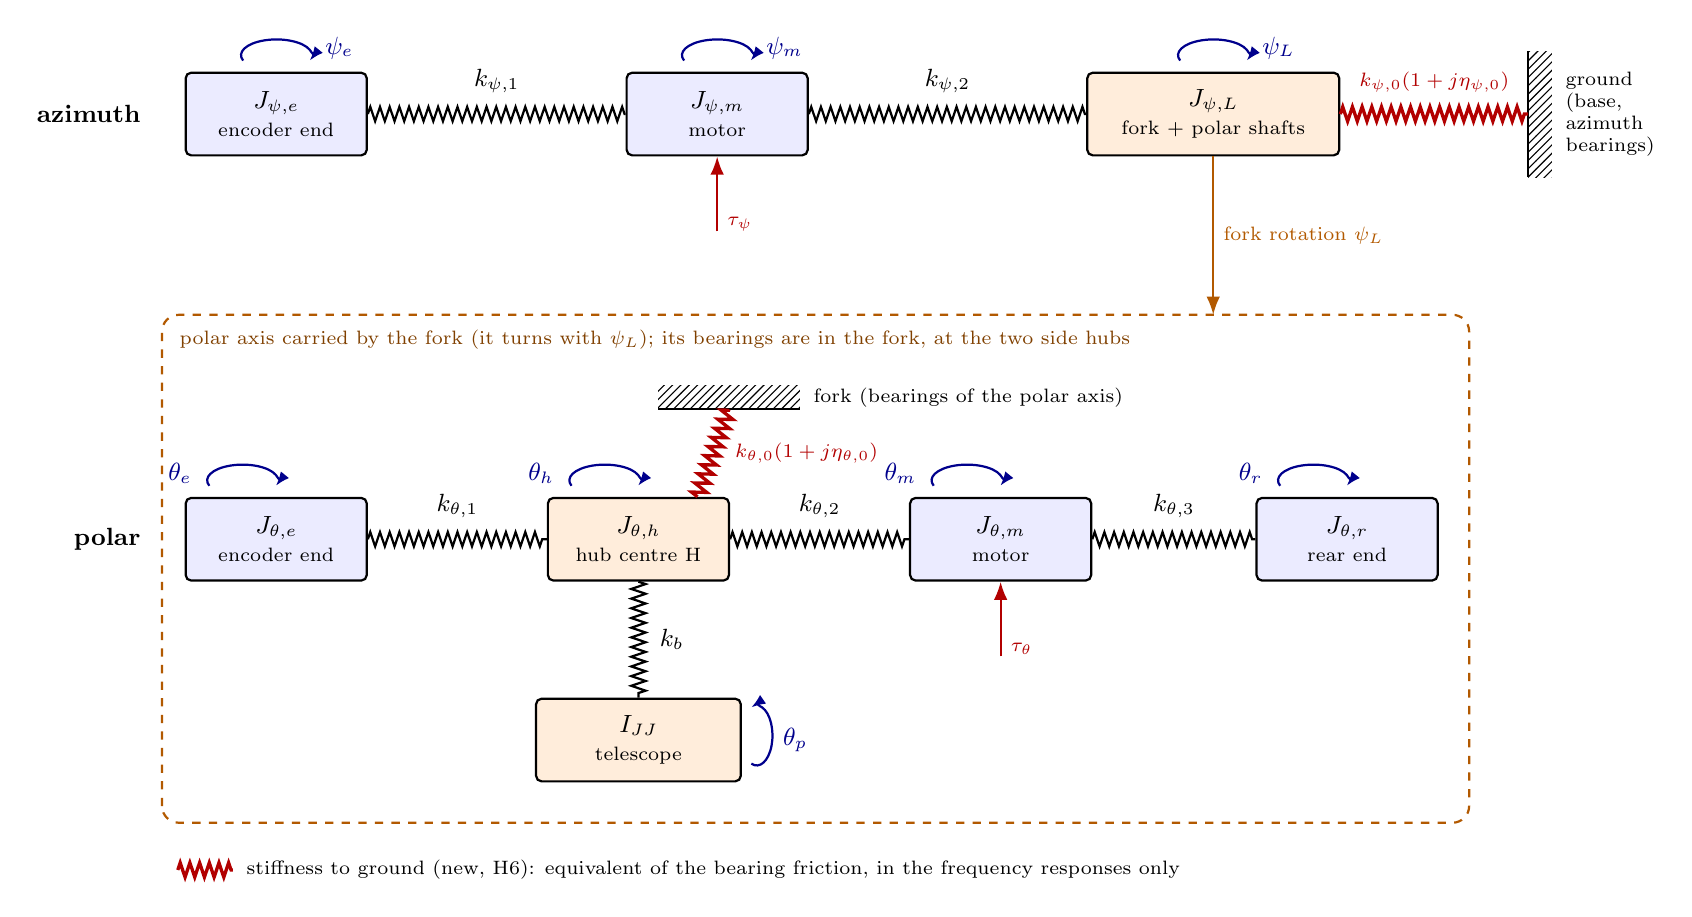
\begin{tikzpicture}[font=\small,
 dof/.style={draw, thick, rounded corners=2pt, minimum width=2.3cm, minimum height=1.05cm, align=center, fill=blue!8},
 spr/.style={decorate, decoration={zigzag, segment length=3.5pt, amplitude=2.6pt}, thick},
 gspr/.style={decorate, decoration={zigzag, segment length=3.5pt, amplitude=2.6pt}, very thick, red!70!black},
 rot/.style={-{Latex[length=1.8mm]}, thick, blue!55!black}]
% ---- azimuth
\node[dof] (pe) at (0,0) {$J_{\psi,e}$\\[-1pt] {\scriptsize encoder end}};
\node[dof] (pm) at (5.6,0) {$J_{\psi,m}$\\[-1pt] {\scriptsize motor}};
\node[dof, fill=orange!14, minimum width=3.2cm] (pL) at (11.9,0) {$J_{\psi,L}$\\[-1pt] {\scriptsize fork + polar shafts}};
\draw[spr] (pe.east) -- node[above=4pt] {$k_{\psi,1}$} (pm.west);
\draw[spr] (pm.east) -- node[above=4pt] {$k_{\psi,2}$} (pL.west);
\foreach \n/\q in {pe/\psi_e, pm/\psi_m, pL/\psi_L} {
  \draw[rot] ($(\n.north)+(-0.42,0.14)$) arc[start angle=200, end angle=-20, x radius=0.45, y radius=0.2];
  \node[blue!55!black, anchor=west] at ($(\n.north)+(0.5,0.3)$) {$\q$};}
\draw[-{Latex}, thick, red!70!black] ($(pm.south)+(0,-0.95)$) -- (pm.south) node[pos=0.1, right, font=\scriptsize] {$\tau_\psi$};
\node[anchor=east] at (-1.6,0) {\textbf{azimuth}};
% ground of the azimuth: the base, which carries the azimuth bearings
\fill[pattern=north east lines] (15.9,-0.8) rectangle (16.2,0.8);
\draw[thick] (15.9,-0.8) -- (15.9,0.8);
\node[anchor=west, font=\scriptsize, align=left] at (16.25,0) {ground\\ (base,\\ azimuth\\ bearings)};
\draw[gspr] (pL.east) -- node[above=4pt, font=\scriptsize] {$k_{\psi,0}(1 + j\eta_{\psi,0})$} (15.9,0);
% ---- polar axis, carried by the fork
\draw[dashed, thick, orange!70!black, rounded corners=6pt] (-1.45,-9.0) rectangle (15.15,-2.55);
\node[anchor=north west, font=\scriptsize, align=left, orange!50!black] at (-1.35,-2.62) {polar axis carried by the fork (it turns with $\psi_L$); its bearings are in the fork, at the two side hubs};
\draw[-{Latex}, thick, orange!70!black] (pL.south) -- node[right, font=\scriptsize] {fork rotation $\psi_L$} (11.9,-2.55);
\node[dof] (te) at (0,-5.4) {$J_{\theta,e}$\\[-1pt] {\scriptsize encoder end}};
\node[dof, fill=orange!14] (th) at (4.6,-5.4) {$J_{\theta,h}$\\[-1pt] {\scriptsize hub centre H}};
\node[dof] (tm) at (9.2,-5.4) {$J_{\theta,m}$\\[-1pt] {\scriptsize motor}};
\node[dof] (tr) at (13.6,-5.4) {$J_{\theta,r}$\\[-1pt] {\scriptsize rear end}};
\node[dof, fill=orange!14, minimum width=2.6cm] (tp) at (4.6,-7.95) {$I_{JJ}$\\[-1pt] {\scriptsize telescope}};
\draw[spr] (te.east) -- node[above=4pt] {$k_{\theta,1}$} (th.west);
\draw[spr] (th.east) -- node[above=4pt] {$k_{\theta,2}$} (tm.west);
\draw[spr] (tm.east) -- node[above=4pt] {$k_{\theta,3}$} (tr.west);
\draw[spr] (th.south) -- node[right=4pt] {$k_b$} (tp.north);
\foreach \n/\q in {te/\theta_e, th/\theta_h, tm/\theta_m, tr/\theta_r} {
  \draw[rot] ($(\n.north)+(-0.85,0.14)$) arc[start angle=200, end angle=-20, x radius=0.45, y radius=0.2];
  \node[blue!55!black, anchor=east] at ($(\n.north)+(-0.95,0.3)$) {$\q$};}
\draw[rot] ($(tp.east)+(0.12,-0.3)$) arc[start angle=-110, end angle=110, x radius=0.2, y radius=0.38];
\node[blue!55!black, anchor=west] at ($(tp.east)+(0.4,0)$) {$\theta_p$};
\draw[-{Latex}, thick, red!70!black] ($(tm.south)+(0,-0.95)$) -- (tm.south) node[pos=0.1, right, font=\scriptsize] {$\tau_\theta$};
\node[anchor=east] at (-1.6,-5.4) {\textbf{polar}};
% fork: carries the polar bearings and the polar constraint
\fill[pattern=north east lines] (4.85,-3.75) rectangle (6.65,-3.45);
\draw[thick] (4.85,-3.75) -- (6.65,-3.75);
\node[anchor=west, font=\scriptsize] at (6.7,-3.6) {fork (bearings of the polar axis)};
\draw[gspr] ($(th.north)+(0.75,0)$) -- node[right=4pt, font=\scriptsize] {$k_{\theta,0}(1 + j\eta_{\theta,0})$} (5.75,-3.75);
% ---- legend
\draw[gspr] (-1.25,-9.6) -- (-0.55,-9.6);
\node[anchor=west, font=\scriptsize] at (-0.5,-9.6) {stiffness to ground (new, H6): equivalent of the bearing friction, in the frequency responses only};
\end{tikzpicture}}
\caption{8-DOF model with the stiffness to ground (red). Azimuth: between the fork and the base. Polar: between the hub centre H, between the two bearing seats, and the fork. Boxes are lumped inertias (one degree of freedom each, blue arrows), black zigzags the equivalent elements of Section~\ref{subsec:8dof}.}\label{fig:ground_scheme}\end{figure}
\paragraph{Newton--Euler equations with the constraint.} With the constraint torques $T_{\psi,0}$ (fork on the ground) and $T_{\theta,0}$ (hub on the fork), the equations of the 8-DOF model of Section~\ref{subsec:8dof} become, one per degree of freedom,
\begin{gather}
(\psi_e)\quad J_{\psi,e}\,\ddot\psi_e = -T_{\psi,1} - b_{\psi,e}\dot\psi_e,\\
(\psi_m)\quad J_{\psi,m}\,\ddot\psi_m = \tau_\psi + T_{\psi,1} - T_{\psi,2} - b_{\psi,m}\dot\psi_m,\\
(\psi_L)\quad \bigl[J_{\psi,L} + J^{ax} + J_{\psi,p}(\theta_p)\bigr]\ddot\psi_L + M_{12}(\theta_p)\,\ddot\theta_p + J_{\psi,p}'(\theta_p)\,\dot\psi_L\dot\theta_p + M_{12}'(\theta_p)\,\dot\theta_p^2 = T_{\psi,2} - T_{\psi,0} - b_{\psi,L}\dot\psi_L,\\
(\theta_e)\quad J_{\theta,e}\,\ddot\theta_e = -T_{\theta,1} - b_{\theta,e}\dot\theta_e,\\
(\theta_h)\quad J_{\theta,h}\,\ddot\theta_h = T_{\theta,1} - T_{\theta,2} - T_b - T_{\theta,0} - b_{\theta,h}\dot\theta_h,\\
(\theta_m)\quad J_{\theta,m}\,\ddot\theta_m = \tau_\theta + T_{\theta,2} - T_{\theta,3} - b_{\theta,m}\dot\theta_m,\\
(\theta_r)\quad J_{\theta,r}\,\ddot\theta_r = T_{\theta,3} - b_{\theta,r}\dot\theta_r,\\
(\theta_p)\quad I_{JJ}\,\ddot\theta_p + M_{12}(\theta_p)\,\ddot\psi_L - \tfrac12 J_{\psi,p}'(\theta_p)\,\dot\psi_L^2 = T_b + M_{g,J}(\theta_p),
\end{gather}
with the element torques of Sections~\ref{subsec:ne7} and~\ref{subsec:8dof}. The constraint torques are defined on the linearised model, in the frequency domain, because the hysteretic loss has no causal expression in time:
\begin{gather}
T_{\psi,0}(j\omega) = k_{\psi,0}\,(1 + j\eta_{\psi,0})\,\psi_L(j\omega),\qquad T_{\theta,0}(j\omega) = k_{\theta,0}\,(1 + j\eta_{\theta,0})\,\theta_h(j\omega),\\
\Bigl[-\omega^2\mathbf M_0 + j\omega\mathbf C_0 + \mathbf K_0 + k_{\psi,0}(1 + j\eta_{\psi,0})\,\mathbf e_{\psi_L}\mathbf e_{\psi_L}^{\mathsf T} + k_{\theta,0}(1 + j\eta_{\theta,0})\,\mathbf e_{\theta_h}\mathbf e_{\theta_h}^{\mathsf T}\Bigr]\,\delta\mathbf q(j\omega) = \mathbf E\,\delta\boldsymbol\tau(j\omega),\label{eq:ground_lin}
\end{gather}
with $\mathbf M_0$, $\mathbf C_0$, $\mathbf K_0$ the matrices of the model linearised at $\theta_0$ and $\mathbf e_{\psi_L}$, $\mathbf e_{\theta_h}$ the unit vectors of the two coordinates. Without the telescope the equation of $\theta_p$ disappears, the hub centre plays the role of P, and the values of the test without telescope are used. In the FEM with hub the same terms are added on the azimuth node 9 and on the polar node H.
\paragraph{Values in the model.} The values of Table~\ref{tab:ground}, rounded, are in the section \texttt{ground\_constraint} of the configuration: $k_{\psi,0} = 1418$\,N\,m/rad, $\eta_{\psi,0} = 0.32$ (azimuth, 3.5\,A); $k_{\theta,0} = 164$\,N\,m/rad, $\eta_{\theta,0} = 3.11$ (polar, 12 screws); $k_{\theta,0} = 2172$\,N\,m/rad, $\eta_{\theta,0} = 1.03$ (polar without telescope). They are linear equivalents for the amplitude of each test, and since \eqref{eq:ground_lin} is complex they enter only the frequency responses: poles and zeros of the structure are unchanged and the time-domain simulator does not include them. Figure~\ref{fig:ground} compares H6 with the measurements over the whole band, with the fit of Section~\ref{sec:fit} in the panel titles: below 5\,Hz the error is within about 1.5\,dB on all axes, the polar response without telescope is followed up to about 40\,Hz, and above a few tens of hertz the models are unchanged.
\begin{figure}[H]\centering
\includegraphics[width=\linewidth,height=0.75\textheight,keepaspectratio]{figures/ground_frf.pdf}
\caption{H6 with the stiffness to ground against the measurements: 8-DOF model (blue) and FEM with hub (orange, dashed) at the encoder, the 8-DOF model without the constraint (dotted) for reference, measurement in black.}\label{fig:ground}\end{figure}

%% ---------------------------------------------------------------------------------------------------
\section{Goodness of fit}\label{sec:fit}
To quantify how well each model reproduces the measurements, the fit is computed as in the System Identification Toolbox (L.~Ljung, \emph{System Identification Toolbox User's Guide}, 2014: ``Best Fit'', used by \texttt{compare} and by \texttt{goodnessOfFit} with the NRMSE cost, and reported by \texttt{greyest}), i.e.\ one minus the normalised root mean square error:
\begin{gather}
\mathrm{fit} = 100\left(1 - \frac{\lVert y - \hat y\rVert}{\lVert y - \bar y\rVert}\right)\ \%,\label{eq:fit}
\end{gather}
with $y$ the measured plant of the encoder channel at the measured frequencies (complex, $G(j\omega_k)$), $\hat y$ the model at the same frequencies and $\bar y$ the mean of $y$. 100\,\% is a perfect model, 0\,\% is no better than a constant, and the fit is negative when the model is worse than that. It is computed on all the measured points and in three bands: 1--5\,Hz (stiffness to ground), 5--100\,Hz (load and telescope dynamics) and above 100\,Hz (structural modes). The norm weights each point by the size of the response, so the complex fit is dominated by the largest values (rigid-body line, resonance peaks); Table~\ref{tab:fit_db} gives the same NRMSE computed on the magnitude in dB, $y = 20\log_{10}|G|$, which weights all frequencies alike (magnitude only). The fit of the measurements of each configuration is also given in the output of the model pipeline (\texttt{experimental\_comparison.csv} and the PDF of each results folder).
\begin{table}[H]\centering\scriptsize\setlength{\tabcolsep}{3pt}
\caption{Fit \eqref{eq:fit} of the complex response of the encoder channel [\%], by model version and band [Hz]. $^{a}$ H4 has $k_b$ for 4 screws: against the 12-screw measurement its 5--100\,Hz band is poor by construction.}\label{tab:fit_complex}
\begin{tabular}{lrrrrrrrrrrrr}\toprule
& \multicolumn{4}{c}{azimuth, 3.5\,A} & \multicolumn{4}{c}{polar, 12 screws} & \multicolumn{4}{c}{polar, no telescope} \\ \cmidrule(lr){2-5}\cmidrule(lr){6-9}\cmidrule(lr){10-13}
model & all & 1--5 & 5--100 & $>$100 & all & 1--5 & 5--100 & $>$100 & all & 1--5 & 5--100 & $>$100 \\ \midrule
7-DOF (baseline) & $-582$ & $-141$ & $3$ & $-585$ & $-197$ & $-460$ & $-7$ & $-1$ & $<-999$ & $<-999$ & $<-999$ & $-748$ \\
8-DOF, H4$^{a}$ & $-582$ & $-138$ & $3$ & $-585$ & $-893$ & $-446$ & $<-999$ & $-295$ & $<-999$ & $<-999$ & $<-999$ & $-48$ \\
8-DOF, H6 without ground & $-582$ & $-138$ & $3$ & $-585$ & $-479$ & $-450$ & $-8$ & $<-999$ & $<-999$ & $<-999$ & $<-999$ & $-79$ \\
8-DOF, H6 & $-582$ & $53$ & $-1$ & $-585$ & $-398$ & $53$ & $10$ & $<-999$ & $-46$ & $80$ & $-41$ & $-83$ \\
FEM with hub, H6 & $-282$ & $53$ & $-1$ & $-284$ & $-567$ & $53$ & $10$ & $<-999$ & $-29$ & $80$ & $-41$ & $-49$
\\ \bottomrule
\end{tabular}\end{table}
\begin{table}[H]\centering\scriptsize\setlength{\tabcolsep}{3pt}
\caption{The same NRMSE fit on the magnitude in dB [\%].}\label{tab:fit_db}
\begin{tabular}{lrrrrrrrrrrrr}\toprule
& \multicolumn{4}{c}{azimuth, 3.5\,A} & \multicolumn{4}{c}{polar, 12 screws} & \multicolumn{4}{c}{polar, no telescope} \\ \cmidrule(lr){2-5}\cmidrule(lr){6-9}\cmidrule(lr){10-13}
model & all & 1--5 & 5--100 & $>$100 & all & 1--5 & 5--100 & $>$100 & all & 1--5 & 5--100 & $>$100 \\ \midrule
7-DOF (baseline) & $10$ & $-91$ & $53$ & $-78$ & $-138$ & $-188$ & $44$ & $-285$ & $-344$ & $<-999$ & $-541$ & $-143$ \\
8-DOF, H4$^{a}$ & $10$ & $-89$ & $54$ & $-78$ & $-118$ & $-184$ & $-149$ & $-144$ & $-202$ & $<-999$ & $-258$ & $-14$ \\
8-DOF, H6 without ground & $10$ & $-89$ & $54$ & $-78$ & $-73$ & $-185$ & $19$ & $-158$ & $-203$ & $<-999$ & $-258$ & $-15$ \\
8-DOF, H6 & $23$ & $74$ & $36$ & $-78$ & $-58$ & $68$ & $19$ & $-158$ & $45$ & $64$ & $56$ & $-14$ \\
FEM with hub, H6 & $30$ & $74$ & $36$ & $-58$ & $-49$ & $68$ & $19$ & $-143$ & $45$ & $64$ & $56$ & $-14$
\\ \bottomrule
\end{tabular}\end{table}
\begin{itemize}
\item \textbf{Low band.} The stiffness to ground takes the 1--5\,Hz fit from $\fitAzLowSeven$\,\% to $\fitAzLow$\,\% on the azimuth, from $\fitPolLowSeven$\,\% to $\fitPolLow$\,\% on the polar axis and to $\fitNtLow$\,\% without the telescope.
\item \textbf{Middle band.} The polar axis with the telescope is the weak point: $\fitPolMid$\,\% on the complex response and $\fitPolMidDb$\,\% on the magnitude in H6, because the features between 40 and 250\,Hz are not modelled (Sections~\ref{sec:screws} and~\ref{sec:open}). On the magnitude the polar axis without telescope reaches $\fitNtMidDb$\,\%. On the azimuth the stiffness to ground lowers the magnitude fit of this band (from 54 to $\fitAzMidDb$\,\%): fitted between 1 and 5\,Hz, it keeps the response slightly above the measurement between 5 and 10\,Hz.
\item \textbf{High band and all points.} The complex fit is negative for every version, and so is the magnitude fit above 100\,Hz. The model resonances have the placeholder damping $\zeta = 0.01$ and stand 20--30\,dB above the measured peaks, and the band contains unmodelled modes and the delay of the drive; since the norm is dominated by the largest values, these peaks also dominate the fit on all points. A meaningful global fit requires the modal damping to be identified.
\item \textbf{FEM against reduced model.} The two have the same fit below 100\,Hz; above, the FEM with hub is better on the azimuth, whose second mode is far above the band.
\end{itemize}

%% ---------------------------------------------------------------------------------------------------
\section{Open issues}\label{sec:open}
\begin{enumerate}
\item \textbf{Low-frequency constraint (azimuth and polar).} The positive slope below a few hertz is now represented by the stiffness to ground of Section~\ref{sec:ground}, a linear equivalent of the bearing friction valid at the amplitude of each test. Friction is not linear: the equivalent stiffness depends on the amplitude (azimuth $\gAzK$\,N\,m/rad at 3.5\,A, $\gAzKlow$\,N\,m/rad at 2.36\,A) and on the load (polar $\gPolK$\,N\,m/rad with the telescope, $\gNtK$\,N\,m/rad without), and the constraint is not in the time-domain simulator.
\item \textbf{Polar response between 45 and 200\,Hz.} The measured encoder channel has resonances at about $\fpMeas$ and $\fNineMeas$\,Hz and an antiresonance--resonance pair at $\fzHundredFiftyMeas$ and $\fTwoHundredMeas$\,Hz. The 8-DOF model and the FEM with hub alike have a single pole in this range, at $\fpEightOne$\,Hz, and no further zero below about 500\,Hz, so the physical correspondence is lost. Both put only $J_{sh} \approx 0.034$\,kg\,m$^2$ on the shaft side of $k_b$, so \eqref{eq:twomass} gives a pole at $\fpEightOne$\,Hz; the measured pole at $\fpMeas$\,Hz needs $J_{sh} = \JoneNeed$\,kg\,m$^2$ (Section~\ref{subsec:branch}), i.e.\ part of the telescope moves rigidly with the hub. The connection test (Section~\ref{sec:screws}) shows that this whole band depends on the ring--telescope connection, while the test without telescope matches reasonably well after the ring fit: the discrepancy is attributed to the telescope and its connection (compliance inside the tube or at several attachment points, optics mounts). The weak $8.4$/$9.2$\,Hz pair of the polar measurement is not modelled either.
\item \textbf{Azimuth.} The first resonance is at $\fAzPoleMeas$\,Hz instead of $\fAzPoleFemSeven$\,Hz (FEM) or $\fAzPoleSeven$\,Hz (reduced models): rotor and encoder inertias at nodes 5 and 1 and joint compliances are missing. A pair at 37/45\,Hz has no counterpart.
\end{enumerate}

%% ---------------------------------------------------------------------------------------------------
\section{Next steps}\label{sec:next}
\begin{itemize}
\item \textbf{Finer frequency step.} Repeat one 4-screw and one 12-screw configuration with the 3\,\% step of 16 October (or finer between 30 and 150\,Hz), to resolve the narrow features that appear with 8 and 12 screws.
\item \textbf{Inertia split.} With every connection the resonance after the telescope antiresonance is lower than in the model: measure the telescope tube and the optics with accelerometers to locate the part that moves with the hub ($J_{sh} \approx 0.12$\,kg\,m$^2$ with 4 screws instead of $0.034$), and repeat the two-mass estimate on the 12-screw records once their resonance is resolved.
\item \textbf{Mode near 400\,Hz.} The ring is no longer the limit (Section~\ref{sec:refit}): check the geometry and the joints of the polar shafts between the hub and the rear end (elements 4--10), and the rotor inertia, which set this mode.
\item \textbf{Parameter estimation.} Use the fit \eqref{eq:fit} as the cost of a grey-box estimation in the spirit of \texttt{greyest}: estimate the free parameters ($k_b$, $\kappa_r$, $k_{\psi,0}$, $\eta_{\psi,0}$, $k_{\theta,0}$, $\eta_{\theta,0}$) and the modal damping band by band, starting with the damping, which dominates the fit above 100\,Hz.
\item \textbf{Friction model.} Measure the low-frequency plant at several current amplitudes (and a slow torque--angle loop) to obtain the stiffness and the loss of the constraint against the amplitude, and identify a Dahl or LuGre friction element for the time-domain simulator.
\item \textbf{Repeatability of the preload.} The two 12-screw settings with similar gaps differ: repeat one setting after dismounting and remounting the tube, to separate the effect of the preload from the scatter of the assembly.
\end{itemize}
\end{document}
